\documentclass[dvipsnames]{beamer}
\usepackage[utf8]{inputenc}
\usepackage{listings}
\usepackage{comment}
\usepackage{soul}
%\usepackage{ulem}
\usepackage{subfig}
\setul{}{1pt}
\usepackage[oldenum, olditem]{paralist}
%allow even smaller text
\newcommand\tinytiny{\fontsize{4pt}{3}\selectfont}

\makeatletter
\let\old@lstKV@SwitchCases\lstKV@SwitchCases
\def\lstKV@SwitchCases#1#2#3{}
\makeatother
\usepackage{lstlinebgrd}
\makeatletter
\let\lstKV@SwitchCases\old@lstKV@SwitchCases

\lst@Key{numbers}{none}{%
    \def\lst@PlaceNumber{\lst@linebgrd}%
    \lstKV@SwitchCases{#1}%
    {none:\\%
     left:\def\lst@PlaceNumber{\llap{\normalfont
                \lst@numberstyle{\thelstnumber}\kern\lst@numbersep}\lst@linebgrd}\\%
     right:\def\lst@PlaceNumber{\rlap{\normalfont
                \kern\linewidth \kern\lst@numbersep
                \lst@numberstyle{\thelstnumber}}\lst@linebgrd}%
    }{\PackageError{Listings}{Numbers #1 unknown}\@ehc}}
\makeatother


\graphicspath{{logos/}}


%disclaimer for Sandia. uncomment and the whole blob goes awa @ 50e13125ad7dby
\def\sandid{SAND2020-7263 PE}

% \title{Performance Portability with Kokkos}
\title{The Kokkos Lectures}
\subtitle{Module 1: Introduction, Building and Parallel Executions}

%BAD misuse of author field
\author{Module 1: Introduction, Building and Parallel Dispatch}

\usetheme{kokkos}

\newif\ifshort
\newif\ifmedium
\newif\iffull
\newif\ifnotoverview

\newcommand{\TutorialDirectory}{\texttt{Intro-Full}}
\newcommand{\ExerciseDirectory}[1]{\texttt{Exercises/#1/}}
\newcommand{\TutorialClone}{\texttt{Kokkos/kokkos-tutorials/\TutorialDirectory}}

\definecolor{darkgreen}{rgb}{0.0, 0.5, 0.0}
\definecolor{darkred}{rgb}{0.8, 0.0, 0.0}
\definecolor{orange}{rgb}{0.8, 0.33, 0.0}
\definecolor{purple}{rgb}{0.60, 0.20, 0.80}
\colorlet{bodyColor}{blue!20}
\colorlet{patternColor}{orange!30}
\colorlet{policyColor}{green!30}

% http://tex.stackexchange.com/questions/144448/color-a-text-line-in-a-code-lstlisting
\lstnewenvironment{code}[1][]%
{
  %with txfonts: OT1/txr/m/n/10
  %with default fonts: OT1/cmr/m/n/10
  %\fontfamily{cmr}\selectfont
  %\showthe\font
   \noindent
   \minipage{\linewidth}
   %\vspace{0.5\baselineskip}
   \lstset{mathescape, escapeinside={<@}{@>},
moredelim=**[is][{\btHL[fill=patternColor]}]{@pattern}{@pattern},
moredelim=**[is][{\btHL[fill=red!30]}]{@warning}{@warning},
moredelim=**[is][{\btHL[fill=policyColor]}]{@policy}{@policy},
moredelim=**[is][{\btHL[fill=bodyColor]}]{@body}{@body},
moredelim=**[is][{\btHL[fill=red!30]}]{@warning}{@warning},
moredelim=**[is][\color{black}]{@black}{@black},
moredelim=**[is][\color{blue}]{@blue}{@blue},
moredelim=**[is][\bf]{@bold}{@bold},
moredelim=**[is][\it]{@italic}{@italic},
moredelim=**[is][\color{boldblue}\bf]{@boldblue}{@boldblue},
moredelim=**[is][\color{red}]{@red}{@red},
moredelim=**[is][\color{green}]{@green}{@green},
moredelim=**[is][\color{gray}]{@gray}{@gray},
moredelim=**[is][\color{darkgreen}]{@darkgreen}{@darkgreen},
moredelim=**[is][\color{darkred}]{@darkred}{@darkred},
moredelim=**[is][\color{orange}]{@orange}{@orange},
moredelim=**[is][\color{purple}]{@purple}{@purple},
keywords={},
#1}
}
{
  \endminipage
  %\vspace{1.0\baselineskip}
}

\makeatletter
\newif\ifATOlinebackground
\lst@Key{linebackground}{\tiny}{\def\ATOlinebackground{#1}\global\ATOlinebackgroundtrue}
\makeatother

\lstnewenvironment{shell}[1][]{%
  \global\ATOlinebackgroundfalse
  \lstset{language=sh,%
    showstringspaces=false,
    aboveskip=0pt,
    frame=none,
    numbers=none,
    belowskip=2pt,
    breaklines=true,
    #1,
    }
  %\ifATOlinebackground
  \lstset{linebackgroundcolor={
    \ATOlinebackground
  }}
  %\fi
  }{}

\lstnewenvironment{cmake}[1][]{%
  \global\ATOlinebackgroundfalse
  \lstset{language=sh,%
    showstringspaces=false,
    aboveskip=0pt,
    frame=none,
    numbers=none,
    belowskip=2pt,
    breaklines=true,
    #1,
    }
  %\ifATOlinebackground
  \lstset{linebackgroundcolor={
    \ATOlinebackground
  }}
  %\fi
  }{}

\newcommand{\inlinecode}[1]{{\lstset{basicstyle=\ttfamily,keywordstyle={},showstringspaces=false}\lstinline$#1$}}
\newcommand{\inlineshell}[1]{{\lstset{basicstyle=\ttfamily,keywordstyle={},showstringspaces=false}\lstinline$#1$}}

\setbeamercolor{block title}{fg=white, bg=SandiaLightBlue}
\setbeamercolor{block body}{bg=lightgray}
\setbeamercolor{block title alerted}{fg=white, bg=SandiaRed}
\setbeamercolor{block body alerted}{bg=lightgray}



%\usepackage[texcoord,grid,gridunit=mm,gridcolor=red!10,subgridcolor=green!10]{eso-pic}
\usepackage[absolute,overlay]{textpos}





% http://tex.stackexchange.com/questions/8851/how-can-i-highlight-some-lines-from-source-code

\usepackage{pgf, pgffor}
\usepackage{listings}
\usepackage{lstlinebgrd} % see http://www.ctan.org/pkg/lstaddons

\makeatletter
%%%%%%%%%%%%%%%%%%%%%%%%%%%%%%%%%%%%%%%%%%%%%%%%%%%%%%%%%%%%%%%%%%%%%%%%%%%%%%
%
% \btIfInRange{number}{range list}{TRUE}{FALSE}
%
% Test in int number <number> is element of a (comma separated) list of ranges
% (such as: {1,3-5,7,10-12,14}) and processes <TRUE> or <FALSE> respectively

\newcount\bt@rangea
\newcount\bt@rangeb

\newcommand\btIfInRange[2]{%
    \global\let\bt@inrange\@secondoftwo%
    \edef\bt@rangelist{#2}%
    \foreach \range in \bt@rangelist {%
        \afterassignment\bt@getrangeb%
        \bt@rangea=0\range\relax%
        \pgfmathtruncatemacro\result{ ( #1 >= \bt@rangea) && (#1 <= \bt@rangeb) }%
        \ifnum\result=1\relax%
            \breakforeach%
            \global\let\bt@inrange\@firstoftwo%
        \fi%
    }%
    \bt@inrange%
}
\newcommand\bt@getrangeb{%
    \@ifnextchar\relax%
        {\bt@rangeb=\bt@rangea}%
        {\@getrangeb}%
}
\def\@getrangeb-#1\relax{%
    \ifx\relax#1\relax%
        \bt@rangeb=100000%   \maxdimen is too large for pgfmath
    \else%
        \bt@rangeb=#1\relax%
    \fi%
}

%%%%%%%%%%%%%%%%%%%%%%%%%%%%%%%%%%%%%%%%%%%%%%%%%%%%%%%%%%%%%%%%%%%%%%%%%%%%%%
%
% \btLstHL<overlay spec>{range list}
%
% TODO BUG: \btLstHL commands can not yet be accumulated if more than one overlay spec match.
%
\newcommand<>{\btLstHL}[2]{%
  \only#3{\btIfInRange{\value{lstnumber}}{#1}{\color{#2}\def\lst@linebgrdcmd{\color@block}}{\def\lst@linebgrdcmd####1####2####3{}}}%
}%
\makeatother






% http://tex.stackexchange.com/questions/15237/highlight-text-in-code-listing-while-also-keeping-syntax-highlighting
%\usepackage[T1]{fontenc}
%\usepackage{listings,xcolor,beramono}
\usepackage{tikz}

\makeatletter
\newenvironment{btHighlight}[1][]
{\begingroup\tikzset{bt@Highlight@par/.style={#1}}\begin{lrbox}{\@tempboxa}}
{\end{lrbox}\bt@HL@box[bt@Highlight@par]{\@tempboxa}\endgroup}

\newcommand\btHL[1][]{%
  \begin{btHighlight}[#1]\bgroup\aftergroup\bt@HL@endenv%
}
\def\bt@HL@endenv{%
  \end{btHighlight}%
  \egroup
}
\newcommand{\bt@HL@box}[2][]{%
  \tikz[#1]{%
    \pgfpathrectangle{\pgfpoint{1pt}{0pt}}{\pgfpoint{\wd #2}{\ht #2}}%
    \pgfusepath{use as bounding box}%
    \node[anchor=base west, fill=orange!30,outer sep=0pt,inner xsep=1pt, inner ysep=0pt, rounded corners=3pt, minimum height=\ht\strutbox+1pt,#1]{\raisebox{1pt}{\strut}\strut\usebox{#2}};
  }%
}
\makeatother



\usetikzlibrary{calc}
\usepackage{xparse}%  For \NewDocumentCommand

% tikzmark command, for shading over items
\newcommand{\tikzmark}[1]{\tikz[overlay,remember picture] \node (#1) {};}

\makeatletter
\NewDocumentCommand{\DrawBox}{s O{}}{%
    \tikz[overlay,remember picture]{
    \IfBooleanTF{#1}{%
        \coordinate (RightPoint) at ($(left |- right)+(\linewidth-\labelsep-\labelwidth,0.0)$);
    }{%
        \coordinate (RightPoint) at (right.east);
    }%
    \draw[red,#2]
      ($(left)+(-0.2em,0.9em)$) rectangle
      ($(RightPoint)+(0.2em,-0.3em)$);}
}

\NewDocumentCommand{\DrawBoxWide}{s O{}}{%
    \tikz[overlay,remember picture]{
    \IfBooleanTF{#1}{%
        \coordinate (RightPoint) at ($(left |- right)+(\linewidth-\labelsep-\labelwidth,0.0)$);
    }{%
        \coordinate (RightPoint) at (right.east);
    }%
    \draw[red,#2]
      ($(left)+(-\labelwidth,0.9em)$) rectangle
      ($(RightPoint)+(0.2em,-0.3em)$);}
}

\NewDocumentCommand{\DrawBoxWideBlack}{s O{}}{%
    \tikz[overlay,remember picture]{
    \IfBooleanTF{#1}{%
        \coordinate (RightPoint) at ($(left |- right)+(\linewidth-\labelsep-\labelwidth,0.0)$);
    }{%
        \coordinate (RightPoint) at (right.east);
    }%
    \draw[black,#2]
      ($(left)+(-\labelwidth,0.9em)$) rectangle
      ($(RightPoint)+(0.2em,-0.3em)$);}
}
\makeatother

\usetikzlibrary{positioning}

\usetikzlibrary{shapes}

\hypersetup{
    colorlinks=true,
    linkcolor=blue,
    filecolor=magenta,
    urlcolor=cyan,
}



\shortfalse
\mediumtrue
\fulltrue
\notoverviewtrue

\begin{document}

% \begin{frame}
%   \titlepage
% \end{frame}
% 
%==============================================================================

\begin{frame}{NVIDIA's NVLABS LOGISTICS (1)}

\textbf{\large SOFTWARE FOR LAB}

\vspace{10pt}

\textbf{Remote Desktop Software:} \\
\begin{itemize}
\item {Download NoMachine now for best performance from \\
 \textbf{\ul{www.nomachine.com/download}}}
\item {Alternatively you may use a VNC client or the provided browser-based VNC option}
\end{itemize}

\vspace{10pt}

\textbf{SSH Access Software (optional):}
\begin{itemize}
\item PuTTy for Windows can be downloaded from \textbf{\ul{www.putty.org}}
\item{Alternatively you may use a provided browser-based SSH option}
\end{itemize}

\end{frame}

%==============================================================================

\begin{frame}{NVIDIA's NVLABS LOGISTICS (2)}

\textbf{\Large CONNECTION INSTRUCTIONS}
\begin{itemize}
\item {Navigate to \textbf{\ul{nvlabs.qwiklab.com}}}
\item {Login or create a new account}
\item {Select the \textbf{Instructor-Led Hands-on Labs} Class}
\item {Find the lab called \textbf{Kokkos, ...}, select it, click Select, and finally click Start}
\item {After a short wait, lab instance Connection information will be shown}
\item {Please ask Lab Assistants for help!}
\end{itemize}

\end{frame}

%==============================================================================



\begin{frame}
	\titlepage
\end{frame}


% \begin{frame}{DOE ECP Acknowledgement}

% \textit{
% This research was supported by the Exascale Computing Project (17-SC-20-SC),
% a joint project of the U.S. Department of Energy’s Office of Science and National Nuclear Security Administration,
% responsible for delivering a capable exascale ecosystem, including software, applications, and hardware technology,
% to support the nation’s exascale computing imperative. 
% }

% \end{frame}

%==============================================================================

\begin{frame}{Welcome to Kokkos}

\textbf{Kokkos is C++ Performance Portability}
\begin{scriptsize}
  \begin{itemize} 
	  \item {Write a \textit{single source} implementation using C++}
	  \item {Use a \textit{descriptive} Programming Model}
	  \item {Compile for GPUs and CPUs}
  \end{itemize}
\end{scriptsize}

	\vspace{10pt}

\textbf{Kokkos is Ready for Use}
\begin{scriptsize}
  \begin{itemize} 
	  \item {Well established project since 2012}
	  \item {Major buy-in by DOE National Labs}
	  \item {Well over 100 projects with over 500 developers use Kokkos}
	  \item {Dedicated developer staff at 5 National Labs}
	  \item {Robust support for software stacks: GCC 8+, Clang 8+, NVCC 11+, ROCM 5.2, Intel 19+}
  \end{itemize}
\end{scriptsize}

\end{frame}


\begin{frame}{Welcome to Kokkos}

\textbf{Online Resources}:

\begin{itemize}
	\item \url{https://github.com/kokkos}: 
		\begin{itemize}
			\item Primary Kokkos GitHub Organization
		\end{itemize}
	\item \url{https://github.com/kokkos/kokkos-tutorials/LectureSeries}: 
		\begin{itemize}
			\item{Find these slides}
		\end{itemize}
	\item \url{https://github.com/kokkos/kokkos/wiki}: 
		\begin{itemize}
			\item Wiki including API reference
		\end{itemize}
	\item \url{https://kokkosteam.slack.com}: 
		\begin{itemize}
			\item Slack channel for Kokkos.
			\item Please join: fastest way to get your questions answered.
			\item Can whitelist domains, or invite individual people. Email: crtrott@sandia.gov
		\end{itemize}
\end{itemize}

\end{frame}


%==============================================================================

\begin{frame}{Lecture Series Outline}

\begin{itemize}
	\item 07/17 Module 1: Introduction, Building and Parallel Dispatch 
	\item 07/24 Module 2: Views and Spaces
	\item 07/31 Module 3: Data Structures + MultiDimensional Loops
	\item 08/07 Module 4: Hierarchical Parallelism
	\item 08/14 Module 5: Tasking, Streams and SIMD
	\item 08/21 Module 6: Internode: MPI and PGAS
	\item 08/28 Module 7: Tools: Profiling, Tuning and Debugging
	\item 09/04 Module 8: Kernels: Sparse and Dense Linear Algebra
        \item 09/11 Reserve Day
\end{itemize}
\end{frame}

\begin{frame}{What to Expect}

\textbf{Lectures}
\begin{itemize}
	\item Typically 90 minutes of lecture
	\item Submodules have associated exercise as homework
	\item Typically 2-3 Exercises per lecture
	\item Exercises will be talked through at next meeting.
\end{itemize}

	\vspace{10pt}

\textbf{Exercises}
\begin{itemize}
	\item Exercises are small codes with places to do modifications.
	\item Access to GPUs helpful for most of them, but most can be done on pure CPU systems.
	\item Only dependent on standard compilers (e.g. Clang, NVCC)
	\item Office hours on Tuesdays 3-5 PM Eastern Time (potentially with AWS access).
        \item Ongoing support at \url{https://kokkosteam.slack.com}
\end{itemize}
\end{frame}

\begin{frame}{Module 1}
  \begin{block}{Introduction}
    What is Kokkos? Who is behind it? Why should you use it?
  \end{block}

  \begin{block}{Parallel Dispatch}
    Pattern, Policy and Body: how to parallelize simple code with Kokkos.
  \end{block}

  \begin{block}{Building}
    What do you need to build Kokkos and Apps? How to integrate into your build system?
  \end{block}

\end{frame}



% \begin{frame}{DOE ECP Acknowledgement}

% \textit{
% This research was supported by the Exascale Computing Project (17-SC-20-SC),
% a joint project of the U.S. Department of Energy’s Office of Science and National Nuclear Security Administration,
% responsible for delivering a capable exascale ecosystem, including software, applications, and hardware technology,
% to support the nation’s exascale computing imperative. 
% }

% \end{frame}

%==============================================================================
\ifnotoverview
\begin{frame}[fragile]

  \vspace{-10pt}

  {\Huge Introduction}

  \vspace{10pt}

  \textbf{Learning objectives:}
  \begin{itemize}
    \item{Why do we need Kokkos}
    \item{The Kokkos Ecosystem}
    \item{The Kokkos Team}
  \end{itemize}

  \vspace{-20pt}

\end{frame}
\fi

\begin{frame}[fragile]{The HPC Hardware Landscape}
  \begin{center}
    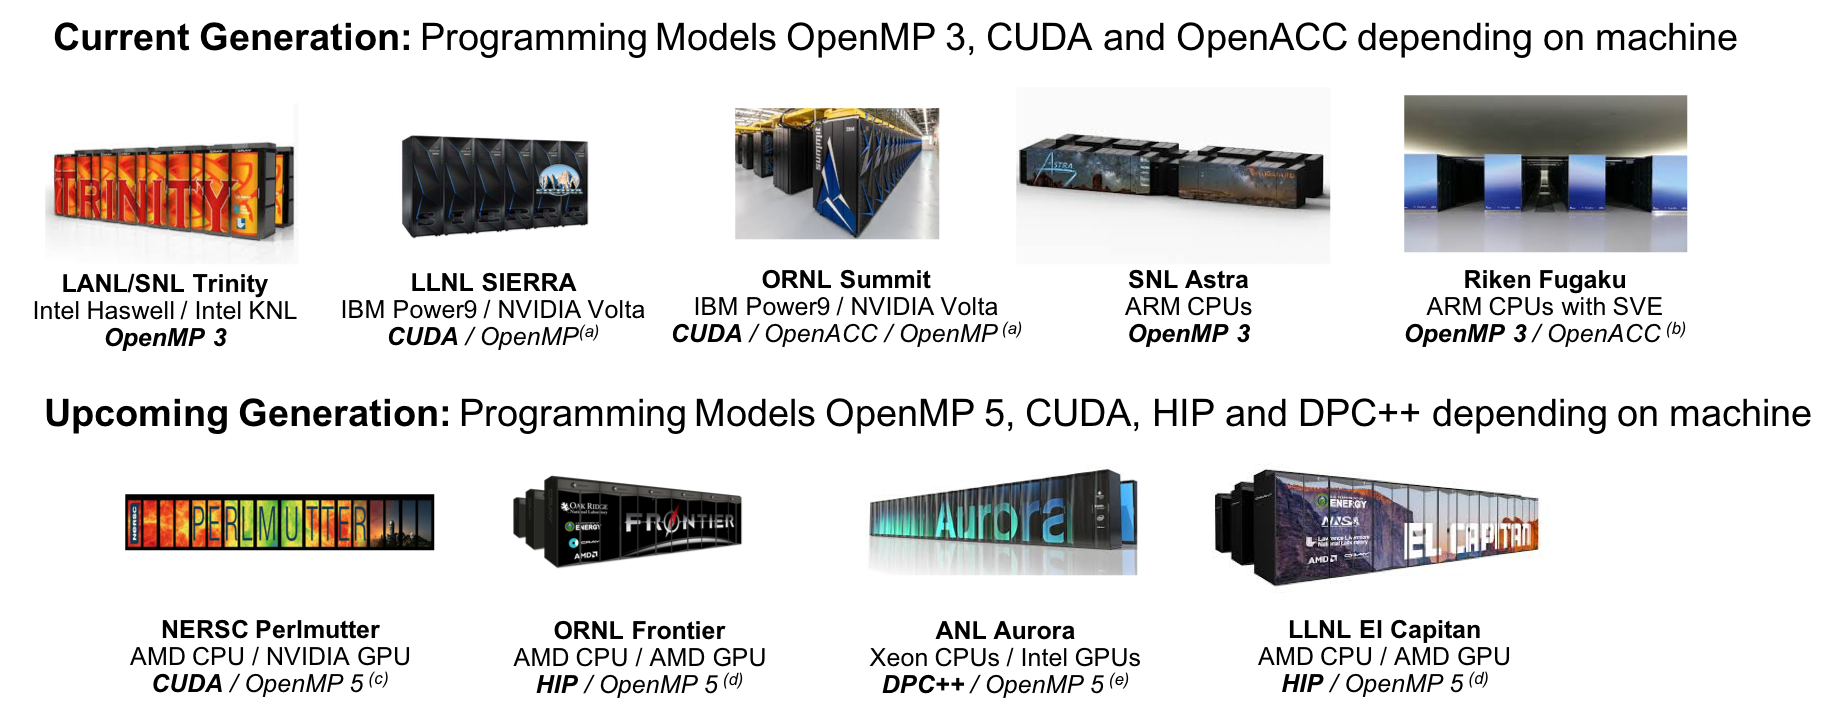
\includegraphics[width=1.05\textwidth]{figures/Architecture-Overview}
  \end{center}

  \begin{scriptsize}
  \emph{(a)} Initially not working. Now more robust for Fortran than C++, but getting better.

  \emph{(b)} Research effort.

  \emph{(c)} OpenMP 5 by NVIDIA.

  \emph{(d)} OpenMP 5 by HPE.

  \emph{(e)} OpenMP 5 by Intel.
  \end{scriptsize}

\end{frame}

\begin{frame}[fragile]{Cost of Coding}

\begin{block}{Industry Estimate}
A full time software engineer writes 10 lines of production code per hour: 20k LOC/year.
\end{block}

	\begin{itemize}
		\item Typical HPC production app: 300k-600k lines
			\begin{itemize}
				\item Sandia alone maintains a few dozen
			\end{itemize}
		\item Large Scientific Libraries:
			\begin{itemize}
				\item E3SM: 1,000k lines
				\item Trilinos: 4,000k lines
			\end{itemize}
	\end{itemize}

	\textbf{Conservative estimate:} need to rewrite 10\% of an app to switch Programming Model

	\pause

\begin{block}{Software Cost Switching Vendors}
Just switching Programming Models costs multiple person-years per app!
\end{block}

\end{frame}

\begin{frame}[fragile]{What is Kokkos?}
	\begin{itemize}
		\item A C++ Programming Model for Performance Portability
			\begin{itemize}
				\item Implemented as a template library on top CUDA, HIP, OpenMP, ...
				\item Aims to be descriptive not prescriptive
				\item Aligns with developments in the C++ standard
			\end{itemize}
		\item Expanding solution for common needs of modern science and engineering codes
			\begin{itemize}
				\item Math libraries based on Kokkos
				\item Tools for debugging, profiling and tuning
				\item Utilities for integration with Fortran and Python
			\end{itemize}
		\item It is an Open Source project with a growing community
			\begin{itemize}
				\item Maintained and developed at \url{https://github.com/kokkos}
				\item Hundreds of users at many large institutions
			\end{itemize}
	\end{itemize}
\end{frame}

\begin{frame}[fragile]{Kokkos at the Center}
  \begin{center}
    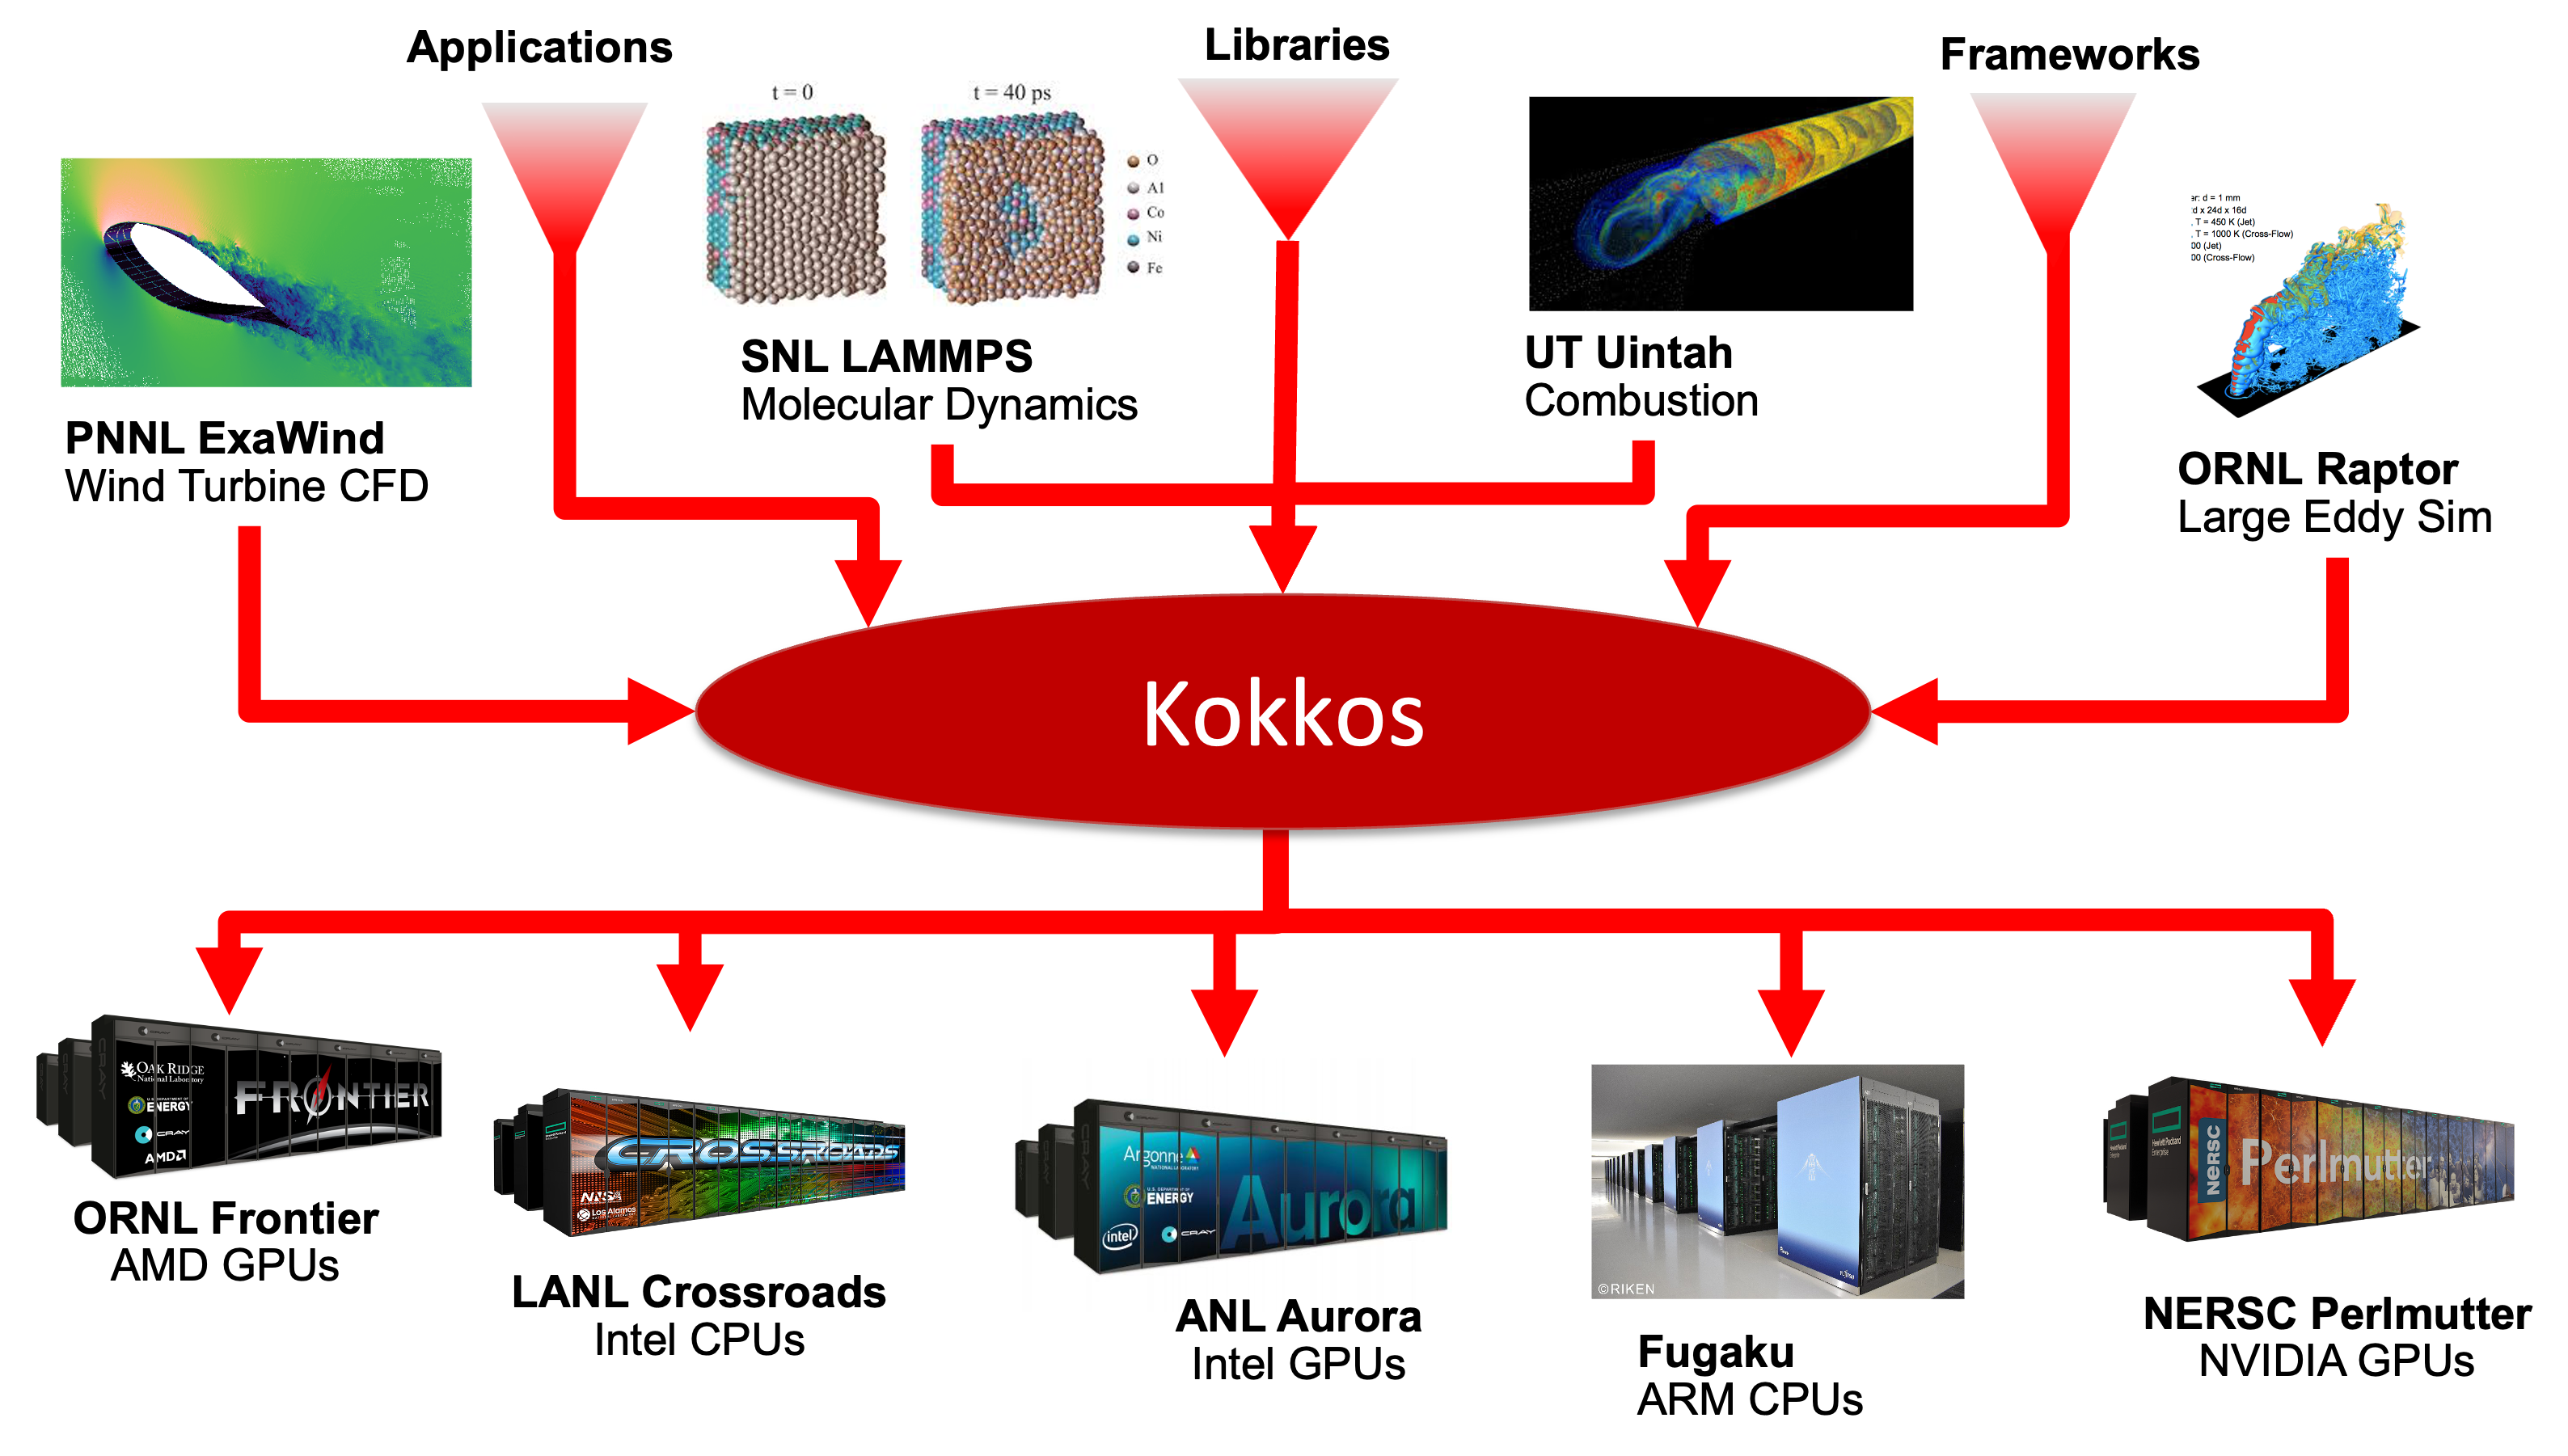
\includegraphics[width=1.05\textwidth]{figures/Kokkos-In-The-Middle-2024}
  \end{center}
\end{frame}

\begin{frame}[fragile]{The Kokkos Ecosystem}
  \begin{center}
    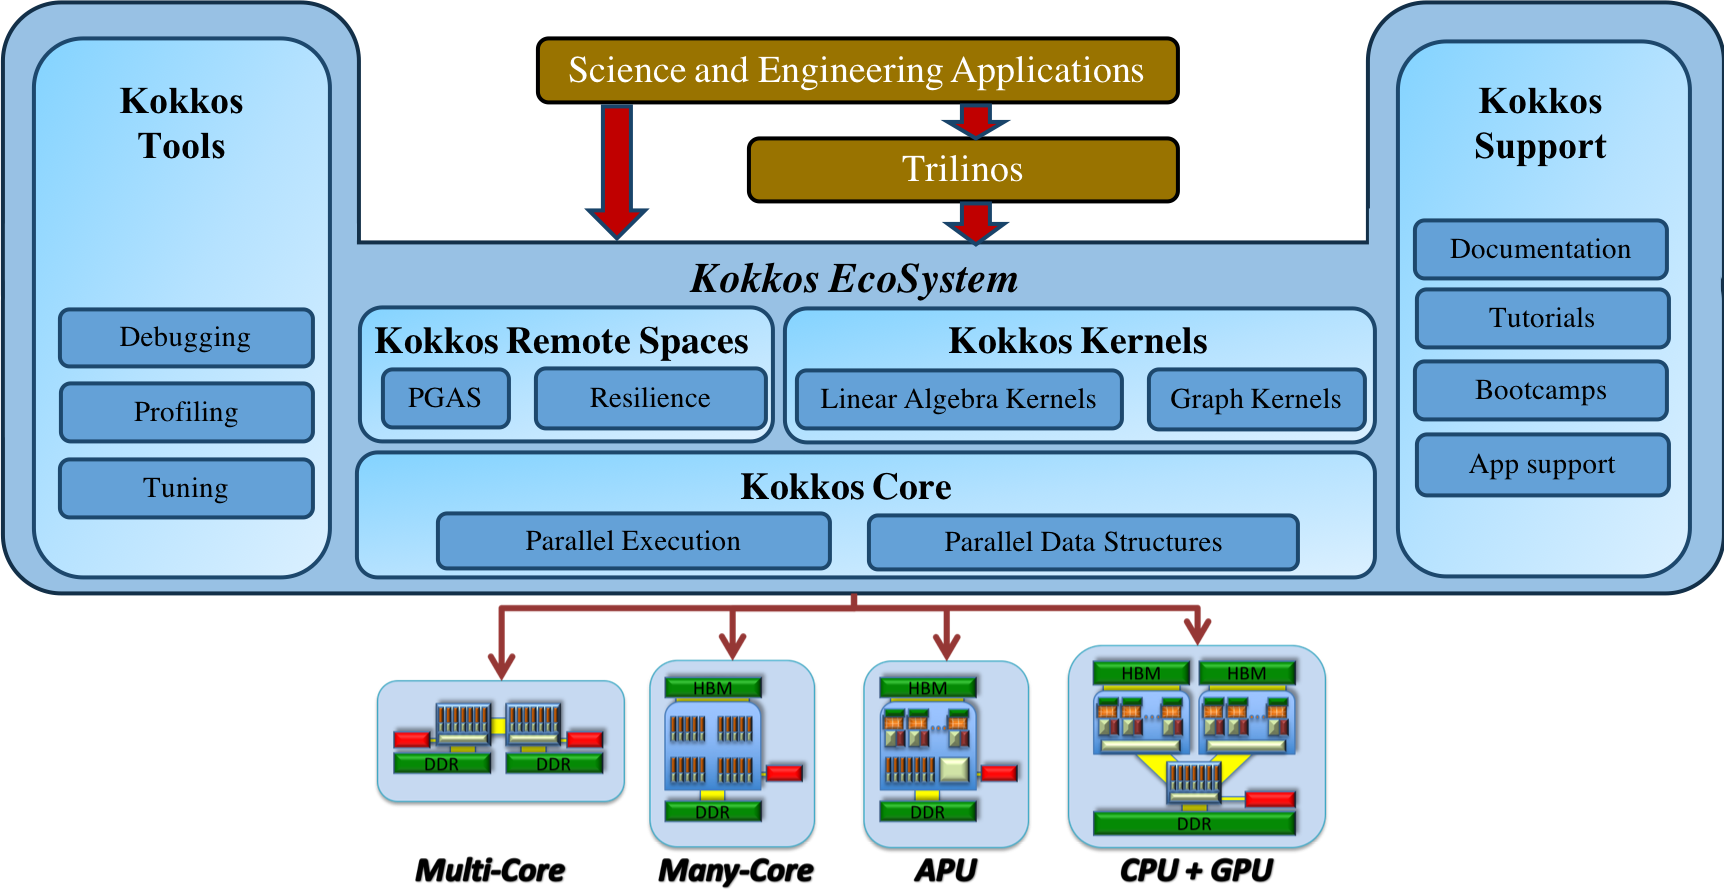
\includegraphics[width=1.05\textwidth]{figures/kokkos-eco-system}
  \end{center}
\end{frame}

\begin{frame}[fragile]{The Kokkos Team}
  \begin{center}
    
\includegraphics[width=0.9\textwidth]{figures/Kokkos-Team-2024}
  \end{center}
\end{frame}


\begin{frame}[fragile]{Kokkos and the C++ Standard}
  \textbf{Kokkos helps improve ISO C++}


	\vspace{-25pt}
\begin{center}                                                                                                                                    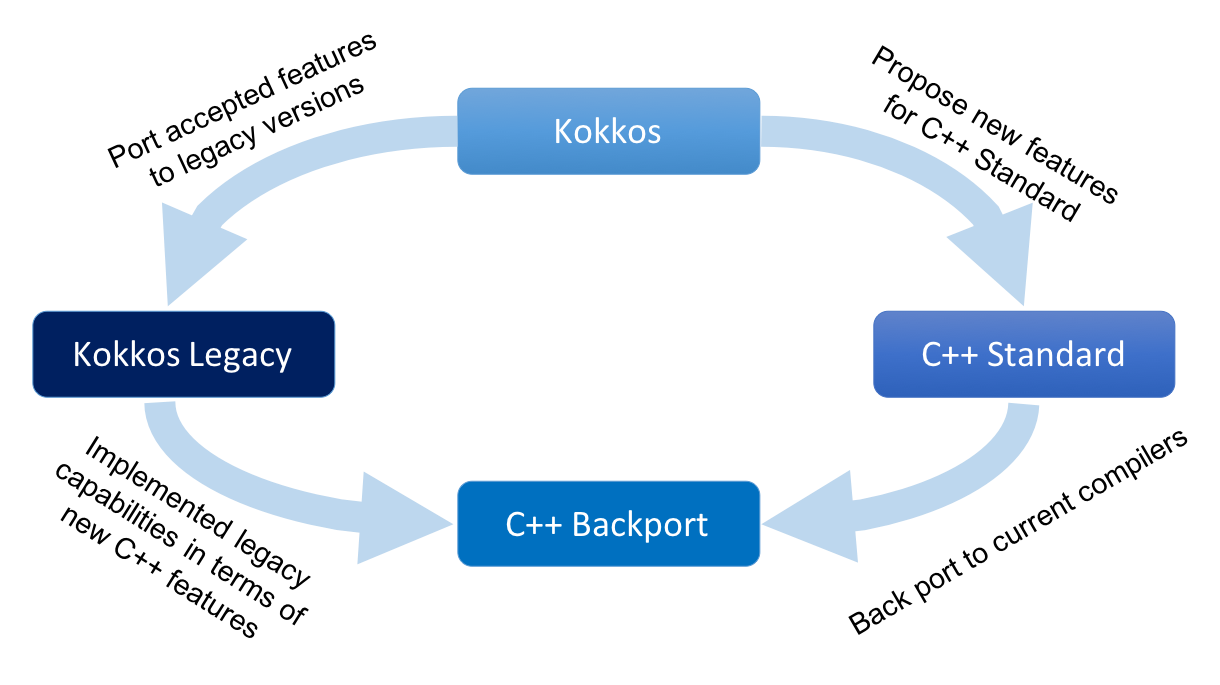
\includegraphics[width=1.05\textwidth]{figures/kokkos-cpp-standard}
\end{center}

	\vspace{-25pt}
\textit{Ten current or former Kokkos team members are members of the ISO C++ standard committee.}
\end{frame}

\iffull
\begin{frame}[fragile]{C++20 std::atomic\_ref}
	\textbf{C++11 std::atomic insufficient for HPC}
	\begin{itemize}
           \item Objects, not functions, with only atomic access
	   \item Can't use non-atomic access in one operation, and then atomic access in the next
	\end{itemize}

	\textbf{C++20 std::atomic\_ref adds atomic capabilites as in Kokkos}
	\begin{itemize}
		\item Can wrap standard allocations.
		\item Works also for sizes which can't be done lock-free (e.g. \texttt{complex$<$double$>$})
		\item Atomic operations on reasonably arbitrary types
	\end{itemize}

  \begin{code}[linebackgroundcolor={
      },
      keywords={atomic_add,atomic_ref}, frame=single
    ]
// Kokkos today
Kokkos::atomic_add(&a[i],5.0);

// atomic_ref in ISO C++20
std::atomic_ref(a[i]) += 5.0;
  \end{code}
\end{frame}
\fi

\iffull
\begin{frame}[fragile]{C++23 std::mdspan}
   \textbf{C++ does not provide multi dimensional arrays}
	\begin{itemize}
           \item Every scientific programming language has them: Fortran, Matlab, Python, ... 
	\end{itemize}

	\textbf{C++23 std::mdspan adds Kokkos::View like arrays}
	\begin{itemize}
		\item Reference semantics.
		\item Compile time and runtime extents (also mixed)
		\item Data layouts to allow for adapting hardware specific access patterns. 
		\item Subviews!
	\end{itemize}

  \begin{code}[linebackgroundcolor={
      },
      keywords={View,LayoutLeft,extents,mdspan,dynamic_extent,layout_left}, frame=single
    ]
// Kokkos today
View<float**[5],LayoutLeft> a("A",10,12); a(3,5,1) = 5;

// mdspan in ISO C++23
using ext = extents<int,dynamic_extent,dynamic_extent,5>;
mdspan<float,ext,layout_left> a(ptr,10,12); a[3,5,1]+=5;
  \end{code}

\end{frame}
\fi

\begin{frame}{Kokkos Users}
\textbf{Kokkos has a growing OpenSource Community}

\vspace{0.5cm}
\begin{itemize}
  \item 20 ECP projects list Kokkos as Critical Dependency
    \begin{itemize}
       \item 41 list C++ as critical
       \item 25 list Lapack as critical
       \item 21 list Fortran as critical
    \end{itemize}
  \item Slack Channel: 1.7k members from 100+ institutions
    \begin{itemize}
      \item 15\% Sandia Nat. Lab.
      \item 24\% other US Labs
      \item 22\% universities
      \item 39\% other
    \end{itemize}
  \item GitHub: 1.9k stars
\end{itemize}

\begin{tikzpicture}[remember picture,overlay]
    \node[xshift=-3.5cm,yshift=-6.5cm] at (current page.north east){%
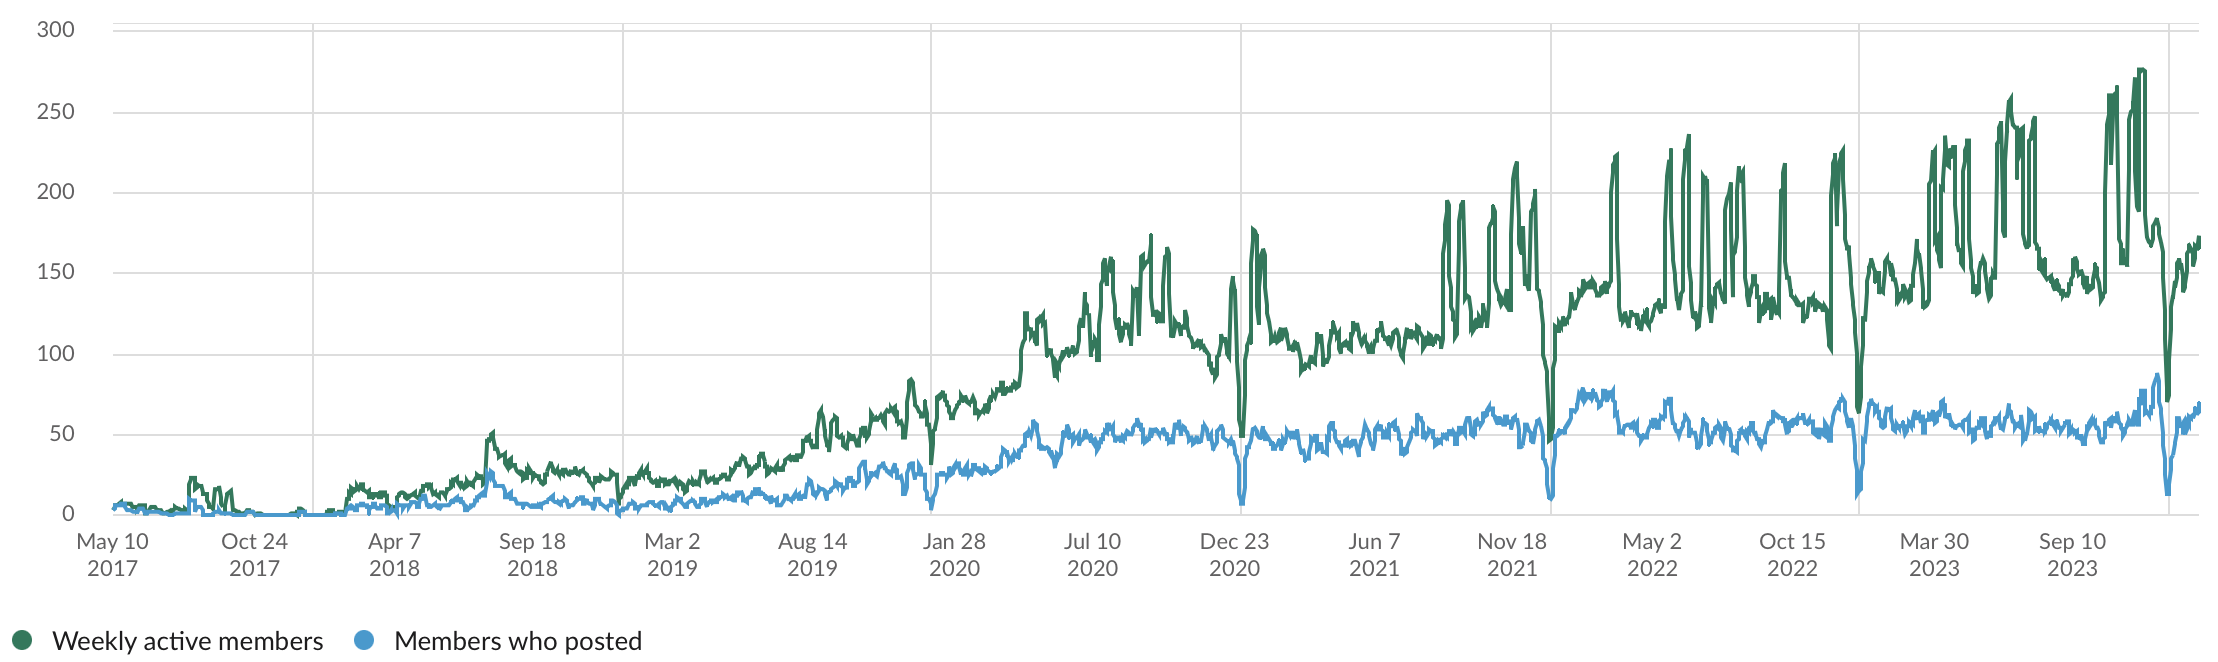
\includegraphics[width=6cm]{figures/KokkosSlack-Users-Feb24}
};
\end{tikzpicture}


\end{frame}



% \begin{frame}{DOE ECP Acknowledgement}

% \textit{
% This research was supported by the Exascale Computing Project (17-SC-20-SC),
% a joint project of the U.S. Department of Energy’s Office of Science and National Nuclear Security Administration,
% responsible for delivering a capable exascale ecosystem, including software, applications, and hardware technology,
% to support the nation’s exascale computing imperative. 
% }

% \end{frame}

%==============================================================================

\begin{frame}{Prerequisites for Tutorial Exercises}

\textbf{Knowledge of C++}:
  class constructors, member variables, member functions, member operators, template arguments

\vspace{10pt}

% \textbf{Using NVIDIA's NVLABS}
%   \begin{itemize}
%   \item Kokkos pre installed in \$\{HOME\}/kokkos
%   \item Exercises pre installed in \$\{HOME\}/\TutorialDirectory
%   \end{itemize}

\vspace{10pt}

\textbf{Using your own {\$\{HOME\}}}
\begin{scriptsize}
  \begin{itemize}
  \item {Git}
  \item {CMake 3.16 (or newer)}
  \item {GCC 8.2 (or newer)}
    \textit{OR} {Intel 19.0.5 (or newer)}
    \textit{OR} {Clang 8.0 (or newer)}
  \item {CUDA nvcc 11.0 (or newer)}
    \textit{AND} {NVIDIA compute capability 6.0 (or newer)}
  \item {git clone \url{https://github.com/kokkos/kokkos-tutorials} \\ \hspace{2pt}  into \path{${HOME}/Kokkos/kokkos-tutorials}}
        \\ \vspace{4pt} \hspace{2pt} Slides are in \\ \hspace{8pt} \path{${HOME}/Kokkos/kokkos-tutorials/LectureSeries}
        \\ \vspace{4pt} \hspace{2pt} Exercises are in \\ \hspace{8pt} \path{${HOME}/Kokkos/kokkos-tutorials/Exercises}
  \end{itemize}
\end{scriptsize}

\end{frame}


\begin{frame}{Prerequisites for Tutorial Exercises}

\textbf{Online Resources}:

\begin{itemize}
	\item \url{https://github.com/kokkos}: Primary Kokkos GitHub Organization
	\item \url{https://kokkos.github.io/kokkos-core-wiki}: Wiki including API reference
	\item \url{https://github.com/kokkos/kokkos-tutorials}: Tutorial exercises
	\item \url{https://kokkosteam.slack.com}: Slack channel for Kokkos
\end{itemize}

\end{frame}


%==============================================================================

\begin{frame}{Lecture Series Objectives}

%  \textbf{Understand Kokkos Programming Model Abstractions}
%  \begin{itemize}
%    \item {What, how and why of \textit{performance portability}}
%    \item {Productivity and hope for future-proofing}
%  \end{itemize}

  %\pause

  \textbf{Kokkos' basic capabilities:}
  \begin{itemize}
    \item {Simple 1D data parallel computational patterns}
    \item {Deciding where code is run and where data is placed}
    \item {Managing data access patterns for performance portability}
    \item {Multidimensional data parallelism}
  \end{itemize}

  %\pause

  \textbf{Kokkos' advanced capabilities:}
  \begin{itemize}
    \item {Thread safety, thread scalability, and atomic operations}
    \item {Hierarchical patterns for maximizing parallelism}
    \item {Task based programming with Kokkos}
  \end{itemize}

  %\pause

  \textbf{Kokkos' tools and Kernels:}
  \begin{itemize}
    \item {How to profile, tune and debug Kokkos code}
    \item {Interacting with Python and Fortran}
    \item {Using Kokkos Kernels math library}
  \end{itemize}

\end{frame}

%==============================================================================

\begin{frame}{Tutorial Takeaways}

  \begin{itemize}
  \item {Kokkos enables \textbf{Single Source Performance Portable Codes}}
  \item {\textbf{Simple things stay simple} - it is not much more complicated than OpenMP}
  \item {\textbf{Advanced performance optimizing capabilities} easier to use with Kokkos than e.g. CUDA or HIP}
  \item {Kokkos provides data abstractions critical for performance portability not available in other programming models \
         \textbf{Controlling data access patterns is key for obtaining performance} }
 \item The \textbf{Kokkos Ecosystem} comes with tools (profiling, debugging, tuning, math libraries, etc.) needed for application development in professional settings
  \end{itemize}

\end{frame}

%==============================================================================

\begin{frame}{Operating assumptions (0)}

  \textbf{Assume you are here because:}
  \begin{itemize}
    \item {Want to use \textbf{all} HPC node architectures; including GPUs}
    \item {Are familiar with \textbf{C++}}
    \item {Want GPU programming to be \textbf{easier}}
    \item {Would like \textbf{portability}, as long as it doesn't hurt performance}
  \end{itemize}
  \textbf{Helpful for understanding nuances:}
  \begin{itemize}
    \item {Are familiar with \textbf{data parallelism}}
    \item {Are familiar with \textbf{OpenMP}}
    \item {Are familiar with \textbf{GPU architecture} and \textbf{CUDA}}
  \end{itemize}

\end{frame}

%==============================================================================

\begin{frame}{Operating assumptions (1)}

  \textbf{Target machine:}
  %\vspace{-10pt}
  \begin{center}
    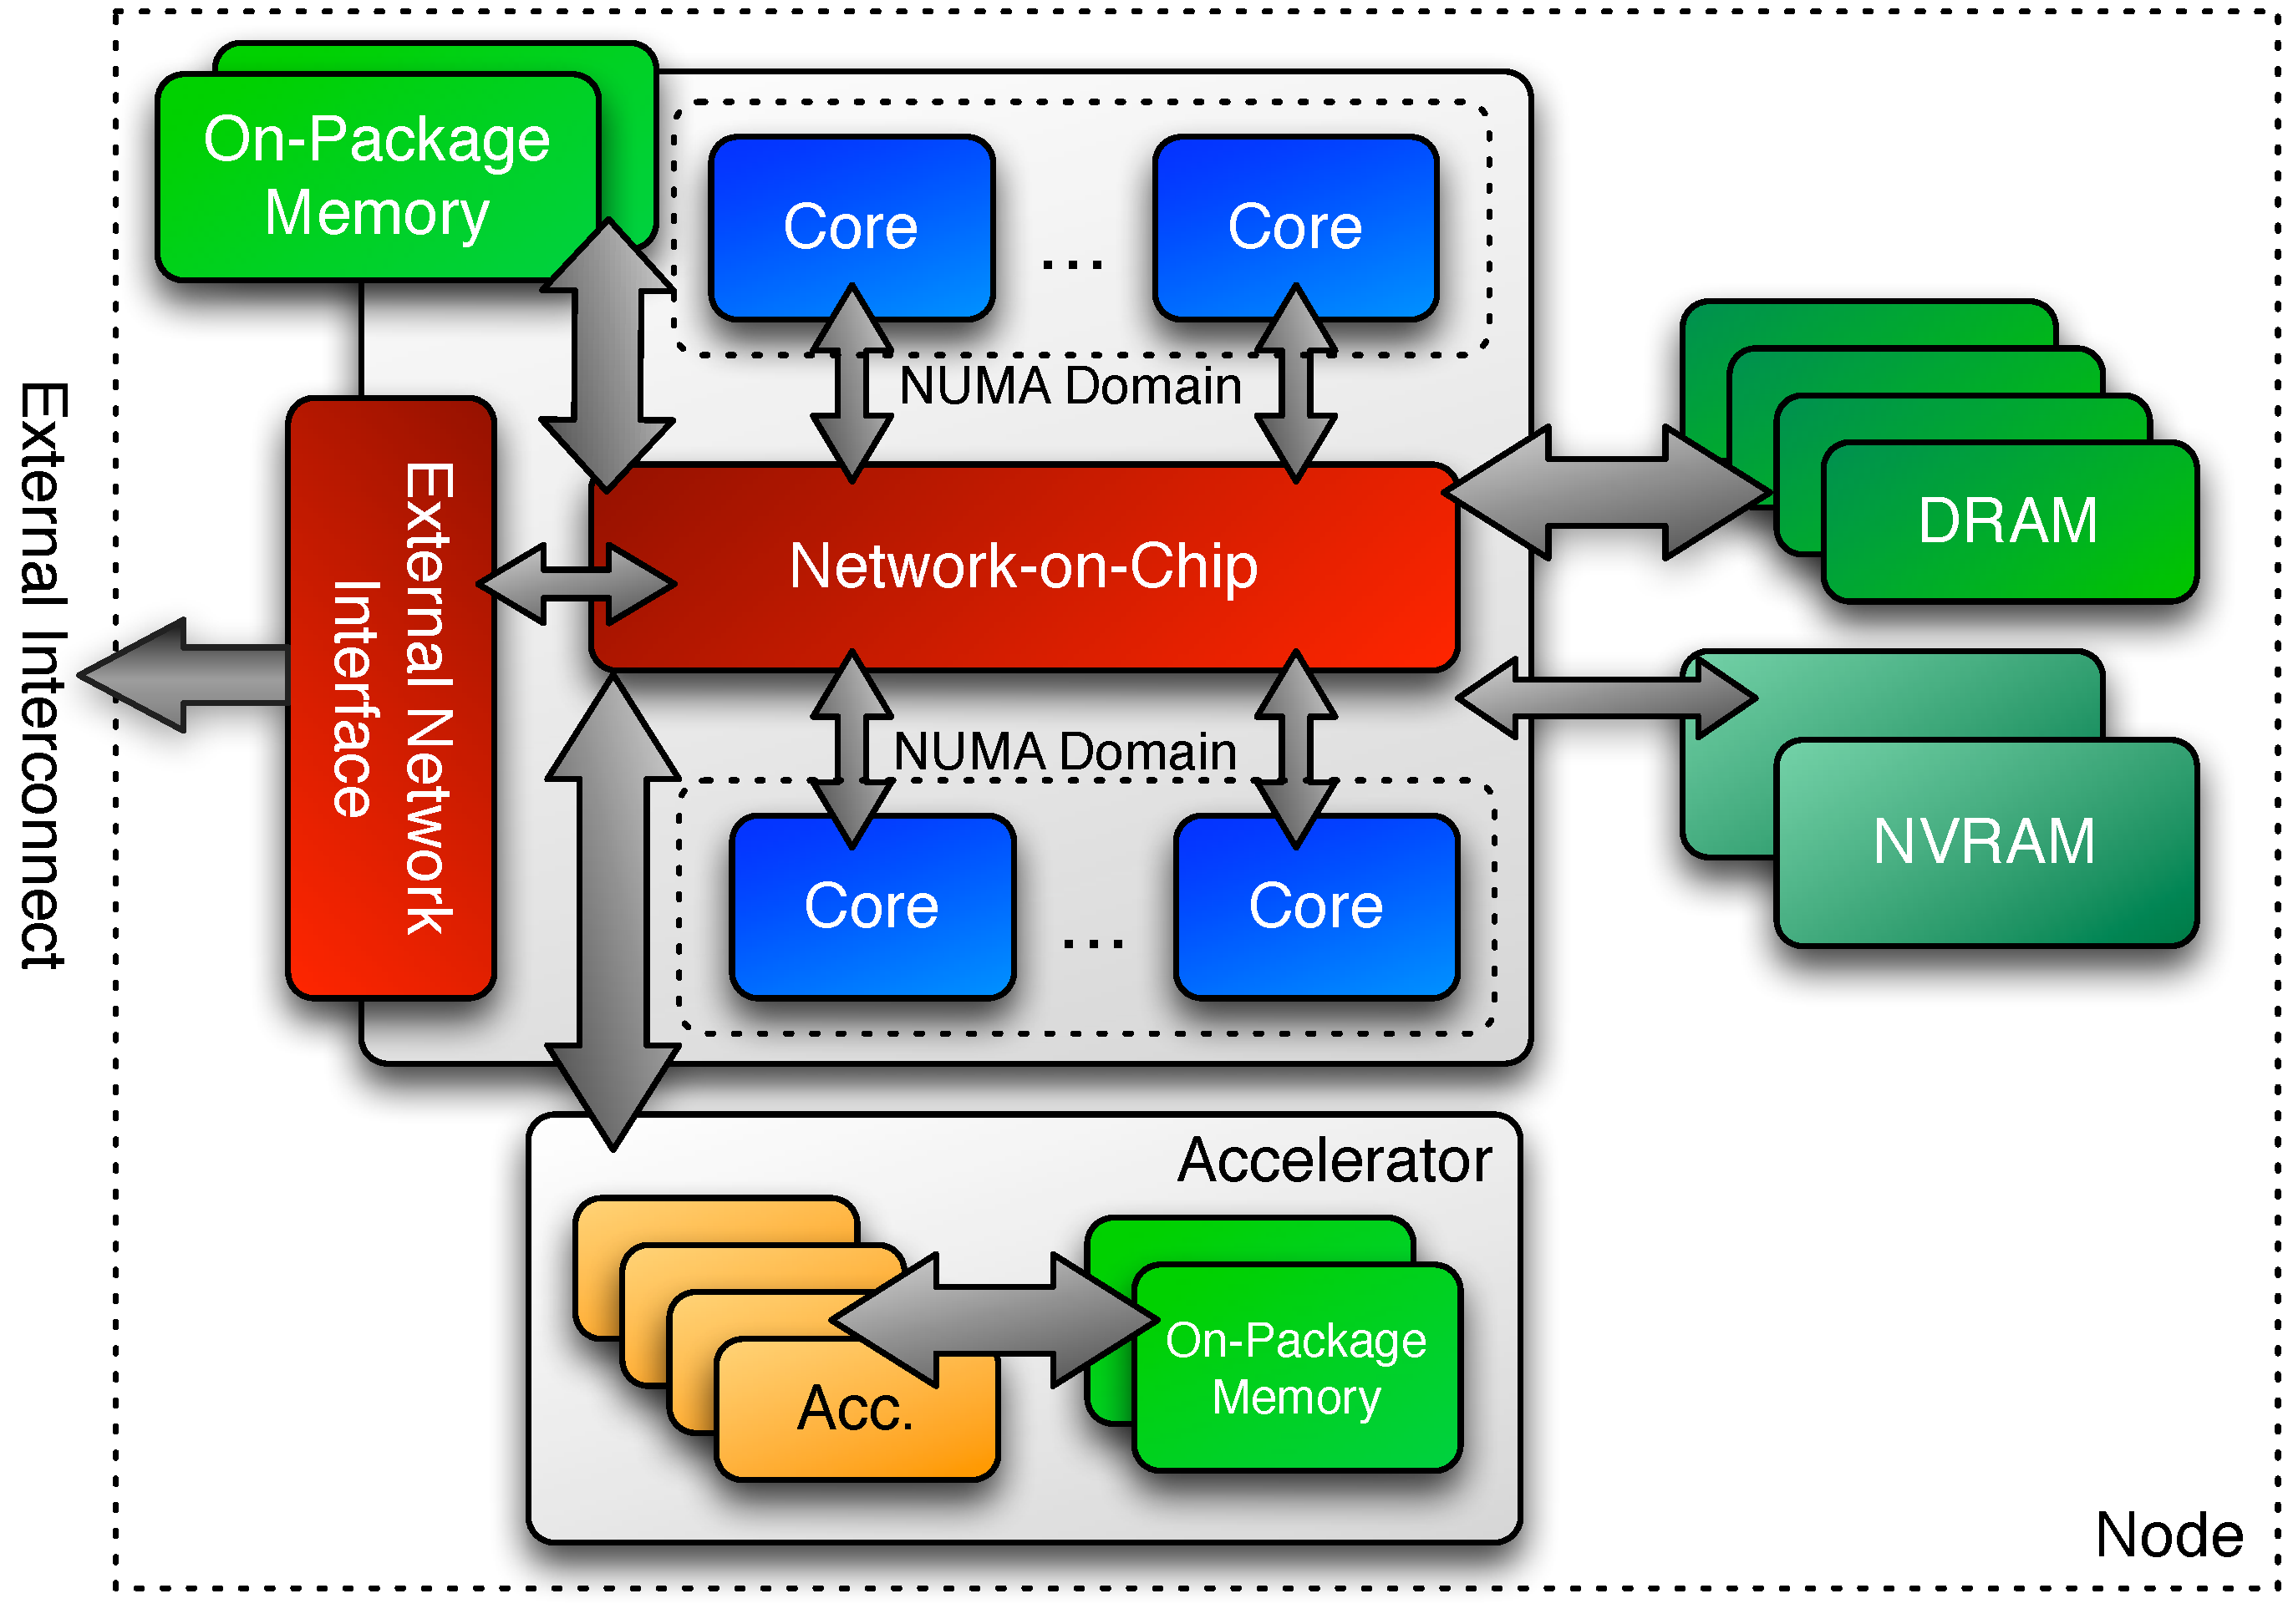
\includegraphics[width=0.80\textwidth]{figures/kokkos-node}
  \end{center}

\end{frame}

%==============================================================================

\begin{frame}[fragile]{Important Point: Performance Portability}

  \begin{block}{Important Point}
    There's a difference between \emph{portability} and
    \\ \emph{performance portability}.
  \end{block}

  \textbf{Example}: implementations may target particular architectures and may not be \emph{thread scalable}. \\
    \hspace{20pt} (e.g., locks on CPU won't scale to 100,000 threads on GPU)

  \pause
  \vspace{5pt}

  \textbf{Goal}: write \textbf{one implementation} which:
  \begin{itemize}
    \item{compiles and \textbf{runs on multiple architectures},}
    \item{obtains \textbf{performant memory access patterns} across architectures,}
    \item{can leverage \textbf{architecture-specific features} where possible.}
  \end{itemize}

  \pause
  \vspace{5pt}
  \textbf{Kokkos}: performance portability across manycore architectures.

  \vspace{5pt}

\end{frame}


%==========================================================================

\begin{frame}[fragile]{}

  {\Huge Concepts for Data Parallelism} 

  \vspace{20pt}

  \textbf{Learning objectives:}
  \begin{itemize}
    \item{Terminology of pattern, policy, and body.}
    \item{The data layout problem.}
  \end{itemize}

  \vspace{-20pt}

\end{frame}

%==========================================================================

\begin{frame}[fragile]{Concepts: Patterns, Policies, and Bodies}

  \begin{onlyenv}<1>
  \begin{code}[linebackgroundcolor={
      }
    ]
for (element = 0; element < numElements; ++element) {
  total = 0;
  for (qp = 0; qp < numQPs; ++qp) {
    total += dot(left[element][qp], right[element][qp]);
  }
  elementValues[element] = total;
}
  \end{code}
  \end{onlyenv}

  \begin{onlyenv}<2->
  \begin{code}[linebackgroundcolor={
        \btLstHL<2>{2-6}{bodyColor}
      }
    ]
@patternfor@pattern (element = @policy0; element < numElements; ++element@policy) {
  total = 0;
  for (qp = 0; qp < numQPs; ++qp) {
    total += dot(left[element][qp], right[element][qp]);
  }
  elementValues[element] = total;
}
  \end{code}
  \end{onlyenv}

  \begin{textblock*}{0.5\textwidth}(0.07\textwidth,0.142\textheight)
    \only<2->{{\footnotesize \color{orange!80} Pattern}}
  \end{textblock*}

  \begin{textblock*}{0.5\textwidth}(0.43\textwidth,0.142\textheight)
    \only<2->{{\footnotesize \color{darkgreen!80} Policy}}
  \end{textblock*}

  \begin{textblock*}{0.5\textwidth}(0.08\textwidth,0.26\textheight)
    \only<2->{\rotatebox{90}{\footnotesize \color{blue!80} Body}}
  \end{textblock*}

  \vspace{0pt}
  \pause

  Terminology:
  \begin{itemize}
    \item{\textbf{Pattern}}: structure of the computations \\
     \hspace{20pt} for, reduction, scan, task-graph, ...
   \item{\textbf{Execution Policy}}: how computations are executed \\
     \hspace{20pt} static scheduling, dynamic scheduling, thread teams, ...
   \item{\textbf{Computational Body}}: code which performs each unit of work; \textit{e.g.}, the loop body \\
  \end{itemize}

  \vspace{2pt}

  \textbf{$\Rightarrow$} The \textbf{pattern} and \textbf{policy} drive the computational \textbf{body}.

  \vspace{-5pt}

\end{frame}

%==========================================================================

\begin{frame}[fragile]{Threading ``Parallel for''}

  What if we want to \textbf{thread} the loop?

  \vspace{5pt}

  \only<1>{\vspace{23pt}}

  \begin{onlyenv}<2->
  \begin{code}[linebackgroundcolor={
      }
    ]
#pragma @policyomp parallel@policy @patternfor@pattern
  \end{code}
  \end{onlyenv}

  \vspace{-12pt}

  \begin{code}[linebackgroundcolor={
        \btLstHL<1-3>{2-6}{bodyColor}
      }
    ]
@patternfor@pattern (element = @policy0; element < numElements; ++element@policy) {
  total = 0;
  for (qp = 0; qp < numQPs; ++qp) {
    total += dot(left[element][qp], right[element][qp]);
  }
  elementValues[element] = total;
}
  \end{code}

  \vspace{2pt}
  \pause

  \hspace{10pt}(Change the \emph{execution policy} from ``serial'' to ``parallel.'')

  \vspace{10pt}
  \pause

  OpenMP is simple for parallelizing loops on multi-core CPUs, \\
  but what if we then want to do this on \textbf{other architectures}? \\
  \vspace{5pt}
  \hspace{10pt}
  Intel PHI \textit{and} NVIDIA GPU \textit{and} AMD GPU \textit{and} ...

  \vspace{10pt}


\end{frame}

%==========================================================================
%==========================================================================

%http://on-demand.gputechconf.com/gtc/2014/presentations/S4438-whats-new-in-openacc-2-openmp-4.pdf
%https://doc.itc.rwth-aachen.de/download/attachments/3474945/OMP4-OpenMP_for_Accelerators.pdf
\begin{frame}[fragile]{``Parallel for'' on a GPU via \texttt{pragmas}}

  \textbf{\ul{Option 1: OpenMP 4.5}}

  \begin{code}[linebackgroundcolor={
        \btLstHL<1->{5,7-9}{bodyColor}
      }
    ]
#pragma @policyomp target@policy @bodydata map(...)@body
#pragma @policyomp teams num_teams(...) num_threads(...)@policy @bodyprivate(...)@body
#pragma @policyomp distribute@policy
@patternfor@pattern (element = @policy0; element < numElements; ++element@policy) {
  total = 0
#pragma @policyomp parallel@policy @patternfor@pattern
  for (qp = 0; qp < numQPs; ++qp)
    total += dot(left[element][qp], right[element][qp]);
  elementValues[element] = total;
}
  \end{code}

  \pause
  \textbf{\ul{Option 2: OpenACC}}

  \begin{code}[linebackgroundcolor={
        \btLstHL<2->{4-7}{bodyColor}
      }
    ]
#pragma @policyacc parallel@policy @bodycopy(...)@body @policynum_gangs(...) vector_length(...)@policy
#pragma @policyacc loop gang vector@policy
@patternfor@pattern (element = @policy0; element < numElements; ++element@policy) {
  total = 0;
  for (qp = 0; qp < numQPs; ++qp)
    total += dot(left[element][qp], right[element][qp]);
  elementValues[element] = total;
}@gray
  \end{code}

\end{frame}

%==========================================================================

\begin{frame}{Portable, but not performance portable}

 \Large A standard thread parallel programming model \\
   \hspace{10pt} \textit{may} give you portable parallel execution \\
   \hspace{10pt} \textit{if} it is supported on the target architecture.

 \vspace{12pt}

 {\Large But what about performance?}

 \vspace{12pt}

 \pause

 {\Large Performance depends upon the computation's
   \\ \textbf{memory access pattern}.}

\end{frame}

%==========================================================================

\begin{frame}[fragile]{Problem: memory access pattern}

  \begin{code}[keywords={}]
@blue#pragma something, opencl, etc.@blue
@grayfor (element = 0; element < numElements; ++element) {
  total = 0;
  for (qp = 0; qp < numQPs; ++qp) {
    for (i = 0; i < vectorSize; ++i) {
@gray@black      total +=
        left[@black@redelement * numQPs * vectorSize +
             qp * vectorSize + i@red@black] *
        right[@black@redelement * numQPs * vectorSize +
              qp * vectorSize + i@red@gray];
    }
  }
  elementValues[element] = total;
}@gray
  \end{code}

  \pause
  \vspace{-2pt}

  \textbf{Memory access pattern problem:} CPU data layout reduces GPU performance by more than 10X.

  \pause
  \vspace{-3pt}

  \begin{block}{Important Point}
    For performance the memory access pattern
    \\  \emph{must} depend on the architecture.
  \end{block}

  \vspace{5pt}

\end{frame}

%==========================================================================

\begin{frame}[fragile]{Kokkos overview}

  How does Kokkos address performance portability?

  \vspace{10pt}

  \textbf{Kokkos} is a \emph{productive}, \emph{portable}, \emph{performant}, shared-memory programming model.

  \begin{itemize}
    \item{is a C++ \textbf{library}, not a new language or language extension.}
    \item{provides \textbf{clear, concise, scalable} parallel patterns.}
    \item{lets you write algorithms once and run on \textbf{many architectures} \\
          \hspace{20pt}e.g. multi-core CPU, GPUs, Xeon Phi, ...}
    \item{\textbf{minimizes} the amount of architecture-specific \textbf{implementation details} users must know.}
    \item{\emph{solves the data layout problem} by using multi-dimensional arrays with architecture-dependent \textbf{layouts}} \\
  \end{itemize}

\end{frame}

%==========================================================================



%==========================================================================

\begin{frame}[fragile]{}

  {\Huge Data parallel patterns}

  \vspace{20pt}

  \textbf{Learning objectives:}
  \begin{itemize}
    \item{How computational bodies are passed to the Kokkos runtime.}
    \item{How work is mapped to execution resources.}
    \item{The difference between \texttt{parallel\_for} and \texttt{parallel\_reduce}.}
    \item{Start parallelizing a simple example.}
  \end{itemize}

  \vspace{-20pt}

\end{frame}

%==========================================================================

\begin{frame}[fragile]{Using Kokkos for data parallel patterns (0)}

  \textbf{\ul{Data parallel patterns and work}}

  \begin{code}[linebackgroundcolor={
        \btLstHL<1->{2}{bodyColor}
      }
    ]
@patternfor@pattern (atomIndex = @policy0; atomIndex < numberOfAtoms; ++atomIndex@policy) {
  atomForces[atomIndex] = calculateForce(...data...);
}
  \end{code}

  Kokkos maps \textbf{work} to execution resources

  \pause

  \begin{itemize}
    \item {each iteration of a computational body is a \textbf{unit of work}.}
    \item {an \textbf{iteration index} identifies a particular unit of work.}
    \item {an \textbf{iteration range} identifies a total amount of work.}
  \end{itemize}

  \pause

  \vspace{0pt}

  \begin{block}{Important concept: Work mapping}
    You give an \textbf{iteration range} and \textbf{computational body} (kernel) \\
    to Kokkos, and Kokkos decides how to map that work to execution resources.
  \end{block}

  \vspace{-10pt}

\end{frame}

%==========================================================================

\begin{frame}[fragile]{Using Kokkos for data parallel patterns (2)}

  \textbf{How are computational bodies given to Kokkos?}

  \vspace{6pt}
  \pause

  \hspace{10pt} As \textbf{functors} or \textit{function objects}, a common pattern in C++.

  \pause
  \vspace{10pt}

  Quick review, a \textbf{functor} is a function with data. Example:
  \begin{code}[keywords={}, frame=single]
struct @darkredParallelFunctor@darkred {
  ...
  void operator()( <@\emph{a work assignment}@> ) const {
    @body/* ... computational body ... */@body
  ...
};
  \end{code}

\end{frame}

%==========================================================================

\begin{frame}[fragile]{Using Kokkos for data parallel patterns (3)}

  \textbf{How is work assigned to functor operators?}

  \vspace{6pt}
  \pause

  \hspace{10pt} A total amount of work items is given to a Kokkos pattern,
  \begin{code}[keywords={}, frame=single]
@darkredParallelFunctor@darkred @bluefunctor@blue;
@patternKokkos::parallel_for@pattern(@policynumberOfIterations@policy, @bluefunctor@blue);
  \end{code}

  \vspace{0pt}
  \pause

  \hspace{10pt} and work items are assigned to functors one-by-one:

  \begin{code}[keywords={}, frame=single]
@graystruct Functor {
  void operator()(@gray@blackconst int64_t index@black@gray) const {...}
}@gray
  \end{code}

  \pause
  \vspace{5pt}

  \begin{alertblock}{Warning: concurrency and order}
    Concurrency and ordering of parallel iterations is \textit{not} guaranteed by the Kokkos runtime.
  \end{alertblock}

  \vspace{0pt}

\end{frame}

%==========================================================================

\iffull
\begin{frame}[fragile]{Using Kokkos for data parallel patterns (4)}

  \textbf{How is data passed to computational bodies?}

  \vspace{2pt}

  \begin{code}
for (atomIndex = 0; atomIndex < numberOfAtoms; ++atomIndex) {
  @darkgreenatomForces@darkgreen[atomIndex] = calculateForce(@darkred...data...@darkred);
}
  \end{code}

  \vspace{-3pt}

  \begin{code}[keywords={}, frame=single]
@graystruct AtomForceFunctor {
  ...
  void operator()(const int64_t atomIndex) const {@gray
    @darkgreenatomForces@darkgreen[atomIndex] = calculateForce(@darkred...data...@darkred);
  @gray}
  ...
}@gray
  \end{code}
  \pause
  \vspace{5pt}

  How does the body access the data?

  \vspace{-3pt}

  \begin{block}{Important concept}
    A parallel functor body must have access to all the data it needs through the functor's \textbf{data members}.
  \end{block}

\end{frame}
\fi

%==========================================================================

\iffull
\begin{frame}[fragile]{Using Kokkos for data parallel patterns (5)}

  \textbf{\ul{Putting it all together: the complete functor}}:

  \begin{code}[keywords={}, frame=single]
struct AtomForceFunctor {
  <@\emph{ForceType}@> @darkgreen_atomForces;@darkgreen
  <@\emph{DataType}@> @darkred_atomData;@darkred
  AtomForceFunctor(/* args */) {...}
  void operator()(const int64_t atomIndex) const {
    @darkgreen_atomForces@darkgreen[atomIndex] = calculateForce(@darkred_atomData@darkred);
  }
};
  \end{code}

  \vspace{5pt}
  \pause

  \textbf{Q/} How would we \textbf{reproduce serial execution} with this functor?

  \vspace{3pt}

  \begin{code}[keywords={}, frame=single]
for (atomIndex = 0; atomIndex < numberOfAtoms; ++atomIndex){
  @darkgreenatomForces@darkgreen[atomIndex] = calculateForce(@darkreddata@darkred);
}
  \end{code}

  \begin{textblock*}{0.5\textwidth}(0.05\textwidth,0.600\textheight)
    \only<2->{\rotatebox{90}{\textbf{Serial}}}
  \end{textblock*}

  %\vspace{3pt}
  \pause

  \begin{code}[keywords={}, frame=single]
AtomForceFunctor @bluefunctor@blue(@darkgreenatomForces@darkgreen, @darkreddata@darkred);
for (atomIndex = 0; atomIndex < numberOfAtoms; ++atomIndex){
  @bluefunctor@blue(atomIndex);
}
  \end{code}

  \begin{textblock*}{0.5\textwidth}(0.05\textwidth,0.755\textheight)
    \only<3->{\rotatebox{90}{\textbf{Functor}}}
  \end{textblock*}

\end{frame}
\fi

%==========================================================================

\begin{frame}[fragile]{Using Kokkos for data parallel patterns (6)}

  \textbf{\ul{The complete picture}} (using functors):

  \vspace{8pt}

  1.  Defining the functor (operator+data):

  \vspace{0pt}

  \begin{code}[keywords={}, frame=single]
struct AtomForceFunctor {
  <@\emph{ForceType}@> @darkgreen_atomForces;@darkgreen
  <@\emph{DataType}@> @darkred_atomData;@darkred

  AtomForceFunctor(<@\emph{ForceType}@> atomForces, <@\emph{DataType}@> data) :
    @darkgreen_atomForces@darkgreen(atomForces), @darkred_atomData@darkred(data) {}

  void operator()(const int64_t atomIndex) const {
    @body@darkgreen_atomForces@darkgreen[atomIndex] = calculateForce(@darkred_atomData@darkred);@body
  }
}
  \end{code}

  \vspace{5pt}

  2.  \textbf{Executing} in parallel with Kokkos pattern:

  \vspace{-4pt}

  \begin{code}
AtomForceFunctor functor(atomForces, data);
@patternKokkos::parallel_for@pattern(@policynumberOfAtoms@policy, functor);
  \end{code}

\end{frame}

%==========================================================================

\begin{frame}[fragile]{Using Kokkos for data parallel patterns (7)}

  Functors are tedious $\Rightarrow$ \ul{\textbf{C++11 Lambdas} are concise}

  \vspace{5pt}

  \begin{code}[linebackgroundcolor={
        \btLstHL<1->{4-6}{black!15}
      },
      keywords={}, frame=single]
@grayatomForces already exists
data already exists
Kokkos::parallel_for(numberOfAtoms, @gray
    [=] (const int64_t atomIndex) {
    @darkgreenatomForces@darkgreen[atomIndex] = calculateForce(@darkreddata@darkred);
  }
@gray);@gray
  \end{code}

  \pause

  A lambda is not \textit{magic}, it is the compiler \textbf{auto-generating} a \textbf{functor} for you.

  \pause
  \vspace{7pt}

  \begin{alertblock}{Warning: Lambda capture and C++ containers}
    For portability to GPU a lambda must capture by value \texttt{[=]}. \\
    Don't capture containers (\textit{e.g.}, std::vector)
    by value because it will copy the container's entire contents.
  \end{alertblock}

  %\pause
  %$\Rightarrow$ So, {\color{darkgreen}\texttt{atomForces}} must be a pointer (e.g., not a \texttt{std::vector})

\end{frame}

%==========================================================================

\begin{frame}[fragile]{parallel\_for examples}

  \textbf{How does this compare to OpenMP?}

  \vspace{5pt}

  \begin{code}[linebackgroundcolor={
      },
      frame=single
    ]
for (int64_t i = 0; i < N; ++i) {
  /* loop body */
}
  \end{code}

  \begin{code}[linebackgroundcolor={
        \btLstHL<1->{3}{bodyColor}
      },
      frame=single
    ]
#pragma @policyomp parallel@policy @patternfor@pattern
@patternfor@pattern (int64_t i = @policy0; i < N@policy; ++i) {
  /* loop body */
}
  \end{code}

  \begin{code}[linebackgroundcolor={
        \btLstHL<1->{2}{bodyColor}
      },
      frame=single
    ]
@patternparallel_for@pattern(@policyN@policy, [=] (const int64_t i) {
  /* loop body */
});
  \end{code}


  \begin{textblock*}{0.5\textwidth}(0.05\textwidth,0.200\textheight)
    \rotatebox{90}{\textbf{Serial}}
  \end{textblock*}

  \begin{textblock*}{0.5\textwidth}(0.05\textwidth,0.350\textheight)
    \rotatebox{90}{\textbf{OpenMP}}
  \end{textblock*}

  \begin{textblock*}{0.5\textwidth}(0.05\textwidth,0.550\textheight)
    \rotatebox{90}{\textbf{Kokkos}}
  \end{textblock*}


  \begin{block}{Important concept}
    Simple Kokkos usage is \textbf{no more conceptually difficult} than OpenMP, the annotations just go in different places.
  \end{block}

\end{frame}

%==========================================================================

\begin{frame}[fragile]{Scalar integration (0)}

  \textbf{\ul{Riemann-sum-style numerical integration}}:

  \vspace{-20pt}

  \begin{columns}[t,onlytextwidth]
    \column{.50\textwidth}
      \vspace{10pt}
      \[y = \int_{\textcolor{darkred}{lower}}^{\textcolor{blue}{upper}} {\textcolor{darkgreen}{function}}(x)\,dx\]
    \column{.50\textwidth}
      \begin{center}
      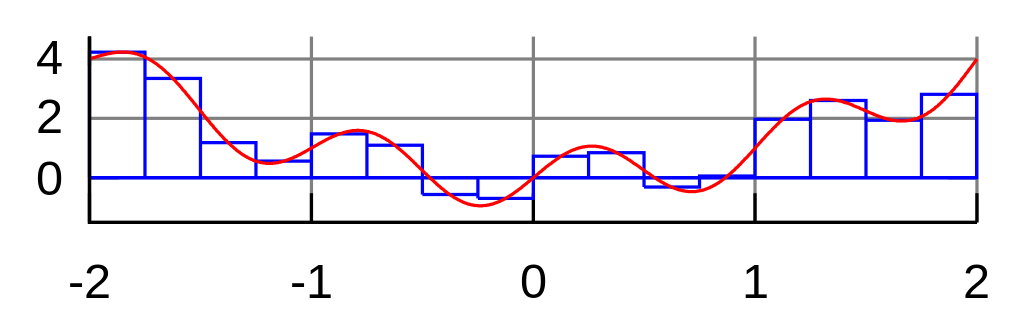
\includegraphics[width=1.0\textwidth]{figures/NumericalIntegration_rectangle}
      \end{center}
      \vspace{-22pt}
      \hspace*{15pt}\hbox{\thinspace{\tinytiny\itshape Wikipedia}}
  \end{columns}

  \vspace{15pt}
  \pause

  \begin{onlyenv}<1>
    \vspace{89pt}
  \end{onlyenv}

  \begin{onlyenv}<2-3>
  \begin{code}[linebackgroundcolor={
      }
    ]
double totalIntegral = 0;
for (int64_t i = 0; i < numberOfIntervals; ++i) {
  const double @orangex@orange =
    <@${\textcolor{darkred}{lower}}$@> + (i/numberOfIntervals) * (<@${\textcolor{blue}{upper}}$@> - <@${\textcolor{darkred}{lower}}$@>);
  const double thisIntervalsContribution = <@${\textcolor{darkgreen}{function}}$@>(@orangex@orange);
  totalIntegral += thisIntervalsContribution;
}
totalIntegral *= dx;
  \end{code}
  \end{onlyenv}

  \begin{onlyenv}<1-3>
    \vspace{10pt}
  \end{onlyenv}

  \begin{onlyenv}<4->
  \begin{code}[linebackgroundcolor={
        \btLstHL<4->{3-6}{bodyColor}
      }
    ]
double totalIntegral = 0;
@patternfor@pattern (int64_t @policyi = 0; i < numberOfIntervals; ++i@policy) {
  const double @orangex@orange =
    <@${\textcolor{darkred}{lower}}$@> + (i/numberOfIntervals) * (<@${\textcolor{blue}{upper}}$@> - <@${\textcolor{darkred}{lower}}$@>);
  const double thisIntervalsContribution = <@${\textcolor{darkgreen}{function}}$@>(@orangex@orange);
  totalIntegral += thisIntervalsContribution;
}
totalIntegral *= dx;
  \end{code}

  \begin{textblock*}{0.5\textwidth}(0.09\textwidth,0.45\textheight)
    \only<4->{\footnotesize {\color{orange!80} Pattern?}}
  \end{textblock*}

  \begin{textblock*}{0.5\textwidth}(0.76\textwidth,0.49\textheight)
    \only<4->{\footnotesize {\color{darkgreen!80} Policy?}}
  \end{textblock*}

  \begin{textblock*}{0.5\textwidth}(0.08\textwidth,0.585\textheight)
    \only<4->{\rotatebox{90}{\footnotesize {\color{blue!80} Body?}}}
  \end{textblock*}
  \pause
  \vspace{10pt}

  \end{onlyenv}

  \begin{onlyenv}<1-2>
    \vspace{10pt}
  \end{onlyenv}

  \begin{onlyenv}<3-4>
  How do we \textbf{parallelize} it?  \textit{Correctly?}
  \end{onlyenv}

\end{frame}

%==========================================================================

\begin{frame}[fragile]{Scalar integration (1)}

  \textbf{\ul{An (incorrect) attempt}}:

  \vspace{5pt}

  \begin{code}[linebackgroundcolor={
        \btLstHL<1->{4-6}{bodyColor}
      },
      frame=single
    ]
double totalIntegral = 0;
@patternKokkos::parallel_for@pattern(@policynumberOfIntervals@policy,
  [=] (const int64_t index) {
    const double x =
      lower + (index/numberOfIntervals) * (upper - lower);
    totalIntegral += function(x);}
  );
totalIntegral *= dx;
  \end{code}

\vspace{15pt}

{\color{red}First problem}: compiler error; cannot increment \texttt{totalIntegral} \\
  \hspace{20pt}(lambdas capture by value and are treated as const!)

\end{frame}

%==========================================================================

\begin{frame}[fragile]{Scalar integration (2)}

  \textbf{\ul{An (incorrect) solution to the (incorrect) attempt}}:

  \vspace{5pt}

  \begin{code}[linebackgroundcolor={
      },
      frame=single
    ]
@graydouble totalIntegral = 0;@gray
@darkreddouble * totalIntegralPointer = &totalIntegral;@darkred
@grayKokkos::parallel_for(numberOfIntervals,
  [=] (const int64_t index) {
    const double x =
      lower + (index/numberOfIntervals) * (upper - lower);@gray
    @darkred*totalIntegralPointer@darkred @gray+= function(x);}
  );
totalIntegral *= dx;@gray
  \end{code}

  \pause
  \vspace{5pt}

  {\color{red}Second problem}: race condition

  \vspace{-7pt}

  \begin{center}
  \begin{tabular}{| c | c | c |}
    \hline
    step & thread 0 & thread 1 \\
    \hline
    0 & load & \\
    \hline
    1 & increment & load \\
    \hline
    2 & write & increment \\
    \hline
    3 & & write \\
    \hline
  \end{tabular}
  \end{center}

  \vspace{-7pt}

\end{frame}

%==========================================================================

\begin{frame}[fragile]{Scalar integration (3)}

  {\color{red}Root problem}: we're using the \textbf{wrong pattern}, \emph{for} instead of \emph{reduction}

  \pause
  \vspace{5pt}

  \begin{block}{Important concept: Reduction}
    Reductions combine the results contributed by parallel work.
  \end{block}

  \vspace{10pt}
  \pause

  How would we do this with \textbf{OpenMP}?

  \vspace{-3pt}

  \begin{code}[linebackgroundcolor={
        \btLstHL<3->{4}{bodyColor}
      }
    ]
double finalReducedValue = 0;
#pragma @policyomp parallel@policy @patternfor reduction@pattern(@pattern+:finalReducedValue@pattern)
@patternfor@pattern (int64_t i = @policy0; i < N; ++i@policy) {
  finalReducedValue += ...
}
  \end{code}

  \pause
  How will we do this with \textbf{Kokkos}?

  \vspace{-3pt}

  \begin{code}[linebackgroundcolor={
        \btLstHL<4->{4}{bodyColor}
      }
    ]
double finalReducedValue = 0;
@patternparallel_reduce@pattern(@policyN@policy, @bodyfunctor@body, finalReducedValue);
  \end{code}

  \vspace{-5pt}

\end{frame}

%==========================================================================

\begin{frame}[fragile]{Scalar integration (4)}

  \ul{\textbf{Example: Scalar integration}}

  \vspace{5pt}

  \begin{code}[linebackgroundcolor={
        \btLstHL<1->{4}{bodyColor}
      },
      frame=single
    ]
double totalIntegral;
#pragma @policyomp parallel@policy @patternfor reduction@pattern(@pattern+:totalIntegral@pattern)
@patternfor@pattern (int64_t i = @policy0; i < numberOfIntervals; ++i@policy) {
  totalIntegral += function(...);
}
  \end{code}

  \begin{code}[linebackgroundcolor={
        \btLstHL<1->{4}{bodyColor}
      },
      frame=single
    ]
double totalIntegral = 0;
@patternparallel_reduce@pattern(@policynumberOfIntervals@policy,
  [=] (const int64_t i, double & valueToUpdate) {
    valueToUpdate += function(...);
  },
  totalIntegral);
  \end{code}

  \begin{textblock*}{0.5\textwidth}(0.05\textwidth,0.22\textheight)
    \rotatebox{90}{\textbf{OpenMP}}
  \end{textblock*}

  \begin{textblock*}{0.5\textwidth}(0.05\textwidth,0.49\textheight)
    \rotatebox{90}{\textbf{Kokkos}}
  \end{textblock*}

  \vspace{-5pt}

  \begin{itemize}
  \item The operator takes \textbf{two arguments}: a work index and a
  value to update.
  \item The second argument is a \textbf{thread-private value} that is
  managed by Kokkos; it is not the final reduced value.
    %by the way, that's what openmp is doing
  \end{itemize}

\end{frame}

%==========================================================================

\iffull
\begin{frame}[fragile]{Amdahl's Law (1)}

  \vspace{-10pt}
  \begin{alertblock}{Warning: Parallelism is NOT free}
    Dispatching (launching) parallel work has non-negligible cost.
  \end{alertblock}

  \pause

  {Simplistic data-parallel performance model: Time = $ \alpha + \frac{\beta * N}{P} $}
  \begin{itemize}
  \item {$\alpha$ = dispatch overhead}
  \item {$\beta$ = time for a unit of work}
  \item {$N$ = number of units of work}
  \item {$P$ = available concurrency}
  \end{itemize}

  \pause

  Speedup = {$P \div {\left( 1 + \frac{\alpha * P}{\beta * N} \right)}$}
  \begin{itemize}
  \item Should have {$\alpha * P \ll \beta * N$}
  \item \textit{All} runtimes strive to minimize launch overhead $\alpha$
  \item Find more parallelism to increase $N$
  \item Merge (fuse) parallel operations to increase $\beta$
  \end{itemize}

  \vspace{-10pt}

\end{frame}
\fi

%==========================================================================

\iffull
\begin{frame}[fragile]{Amdahl's Law (2)}

  \vspace{12pt}

  \textbf{\ul{Results}}:
  {illustrates simple speedup model = {$P \div {\left( 1 + \frac{\alpha * P}{\beta * N} \right)}$}}

  \vspace{-32pt}

  \begin{center}
    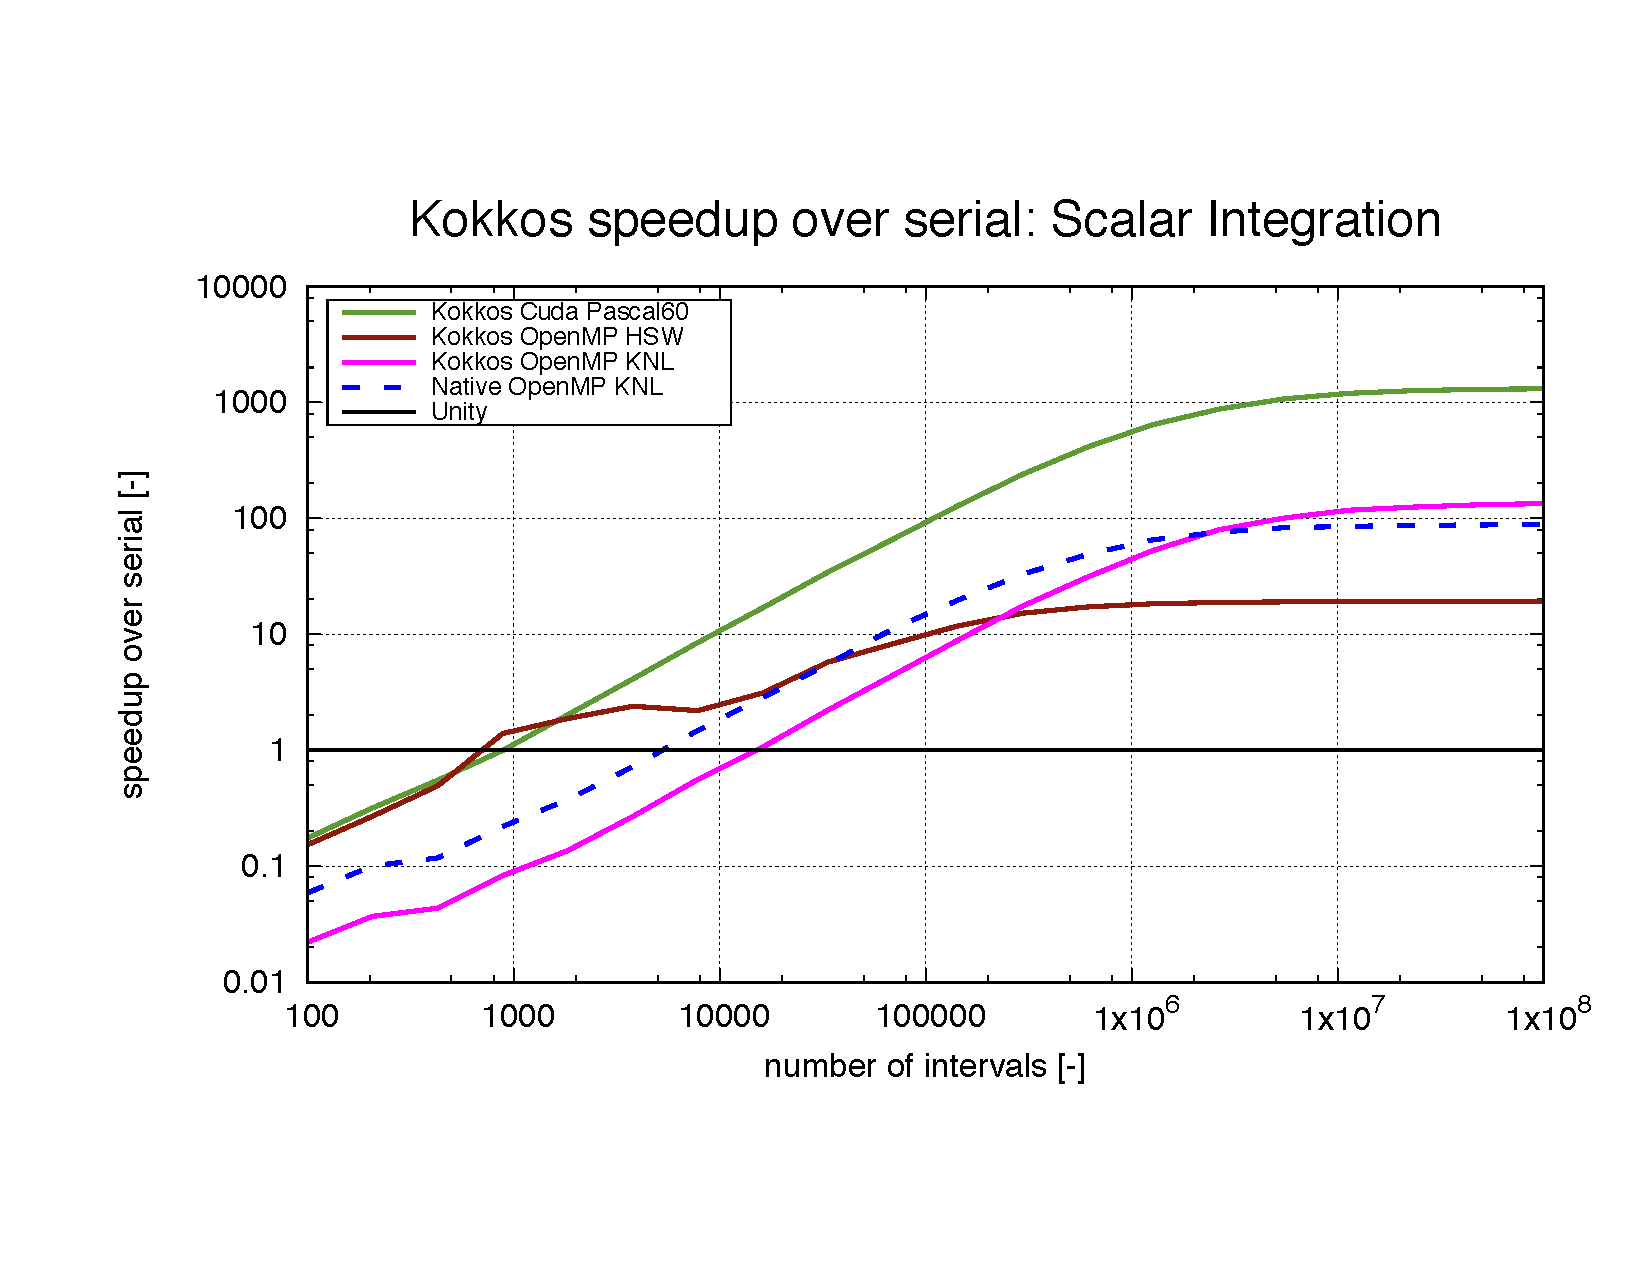
\includegraphics[width=1.00\textwidth]{figures/ScalarIntegration.pdf}
  \end{center}

  \vspace{-24pt}

  \begin{textblock*}{0.5\textwidth}(1.06\textwidth,0.33\textheight)
    \rotatebox{90}{\textbf{Note: log scale}}
  \end{textblock*}

\end{frame}
\fi

%==========================================================================

\begin{frame}[fragile]{Naming your kernels}
  \vspace{-10pt}
  \begin{alertblock}{Always name your kernels!}
     Giving unique names to each kernel is immensely helpful for debugging and profiling. You will regret it if you don't!
  \end{alertblock}
 
  \begin{itemize}
     \item Non-nested parallel patterns can take an optional string argument.
     \item The label doesn't need to be unique, but it is helpful.
     \item Anything convertible to "std::string"
     \item Used by profiling and debugging tools (see Profiling Tutorial)
  \end{itemize}
  \textbf{Example:} 
  \begin{code}[linebackgroundcolor={
        \btLstHL<1->{4}{bodyColor}
      },
      frame=single
    ]
double totalIntegral = 0;
@patternparallel_reduce@pattern("Reduction",@policynumberOfIntervals@policy,
  [=] (const int64_t i, double & valueToUpdate) {
    valueToUpdate += function(...);
  },
  totalIntegral);
  \end{code}
\end{frame}

%==========================================================================

\begin{frame}[fragile]{Recurring Exercise: Inner Product}

  \textbf{Exercise}: Inner product $<y, A * x>$

  \vspace{-10pt}

  \begin{center}
    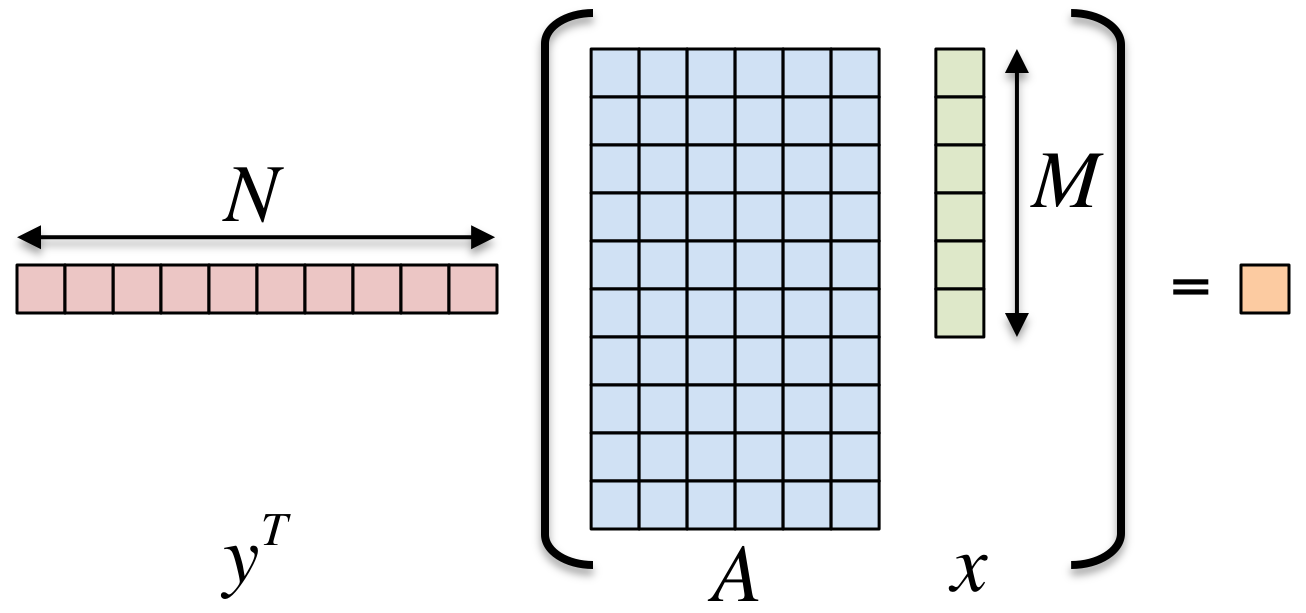
\includegraphics[width=0.80\textwidth]{figures/InnerProductExample_annotated}
  \end{center}

  \vspace{-15pt}

  \textbf{Details}:
  \begin{itemize}
    \item $y$ is $Nx1$, $A$ is $NxM$, $x$ is $Mx1$
    \item We'll use this exercise throughout the tutorial
  \end{itemize}

\end{frame}

%==========================================================================

\begin{frame}[fragile]{Exercise \#1: include, initialize, finalize Kokkos}

  The \textbf{first step} in using Kokkos is to include, initialize, and finalize:

  \begin{code}
#include <Kokkos_Core.hpp>
int main(int argc, char* argv[]) {
  /* ... do any necessary setup (e.g., initialize MPI) ... */
  Kokkos::initialize(argc, argv);
  {
  /* ... do computations ... */
  }
  Kokkos::finalize();
  return 0;
}
  \end{code}

  \vspace{7pt}

  (Optional) Command-line arguments or environment variables:

  \vspace{3pt}

	\begin{tabular}{| p{0.5\textwidth} | p{0.5\textwidth} |}
    \hline
	  \texttt{--kokkos-num-threads=INT} or \texttt{KOKKOS\_NUM\_THREADS} & total number of threads \\
    \hline
	  \texttt{--kokkos-device-id=INT} or \texttt{KOKKOS\_DEVICE\_ID} & device (GPU) ID to use \\
    \hline
  \end{tabular}

\end{frame}

%==========================================================================


\begin{frame}[fragile]{Exercise \#1: Inner Product, Flat Parallelism on the CPU}

  \vspace{5pt}

  \textbf{Exercise}: Inner product $<y, A * x>$

  \vspace{-10pt}

  \begin{center}
    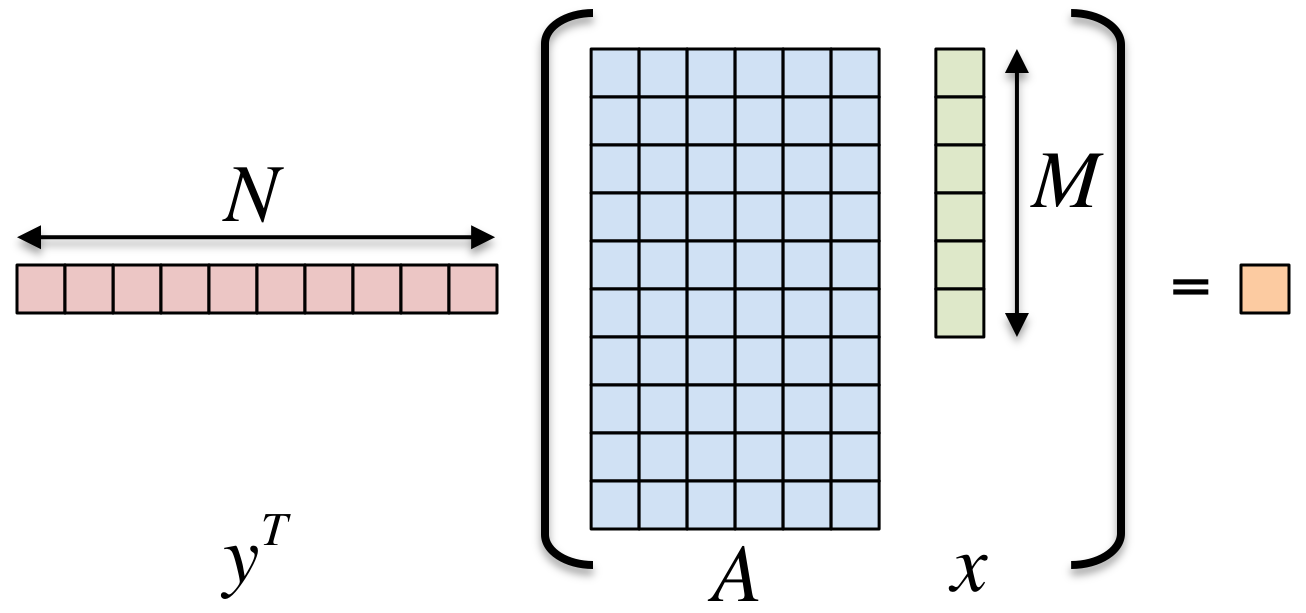
\includegraphics[width=0.65\textwidth]{figures/InnerProductExample_annotated}
  \end{center}

  \vspace{-30pt}

  \textbf{Details}:
  \begin{small}
  \begin{itemize}
\item Location: \ExerciseDirectory{01/Begin}
\item Look for comments labeled with ``EXERCISE''
\item Need to include, initialize, and finalize Kokkos library
\item Parallelize loops with \texttt{parallel\_for} or \texttt{parallel\_reduce}
\item Use lambdas instead of functors for computational bodies.
\item For now, this will only use the CPU.
\end{itemize}
  \end{small}

\end{frame}

%==========================================================================

\begin{frame}[fragile]{Exercise \#1: logistics}

\ul{\textbf{Compiling for CPU}}

\vspace{-3pt}
  \begin{small}
  \begin{code}
  cmake -B build_openmp -DKokkos_ENABLE_OPENMP=ON \
      -DCMAKE_BUILD_TYPE=Release
  cmake --build build_openmp
  \end{code}
  \end{small}

%  \hspace{10pt} {\tiny \url{https://github.com/kokkos/kokkos/wiki/Compiling#table-43-architecture-variables}}

\ul{\textbf{Running on CPU} with OpenMP backend}

\vspace{-3pt}
  \begin{small}
  \begin{code}
  # Set OpenMP affinity
  export OMP_NUM_THREADS=8
  export OMP_PROC_BIND=spread OMP_PLACES=threads
  # Print example command line options:
  ./build_openmp/01_Exercise -h
  # Run with defaults on CPU
  ./build_openmp/01_Exercise
  # Run larger problem
  ./build_openmp/01_Exercise -S 26
  \end{code}
  \end{small}

\ul{\textbf{Things to try:}}
  \begin{small}
  \begin{itemize}
  \itemsep0em
%  \item Vary number of threads
  \item Vary problem size with command line argument -S $s$
  \item Vary number of rows with command line argument -N $n$
  \item Num rows = $2^n$, num cols = $2^m$, total size = $2^s == 2^{n+m}$
  \end{itemize}
  \end{small}
\end{frame}

%==========================================================================

\begin{frame}[fragile]{Exercise \#1 results}

  \vspace{-10pt}

  \begin{center}
    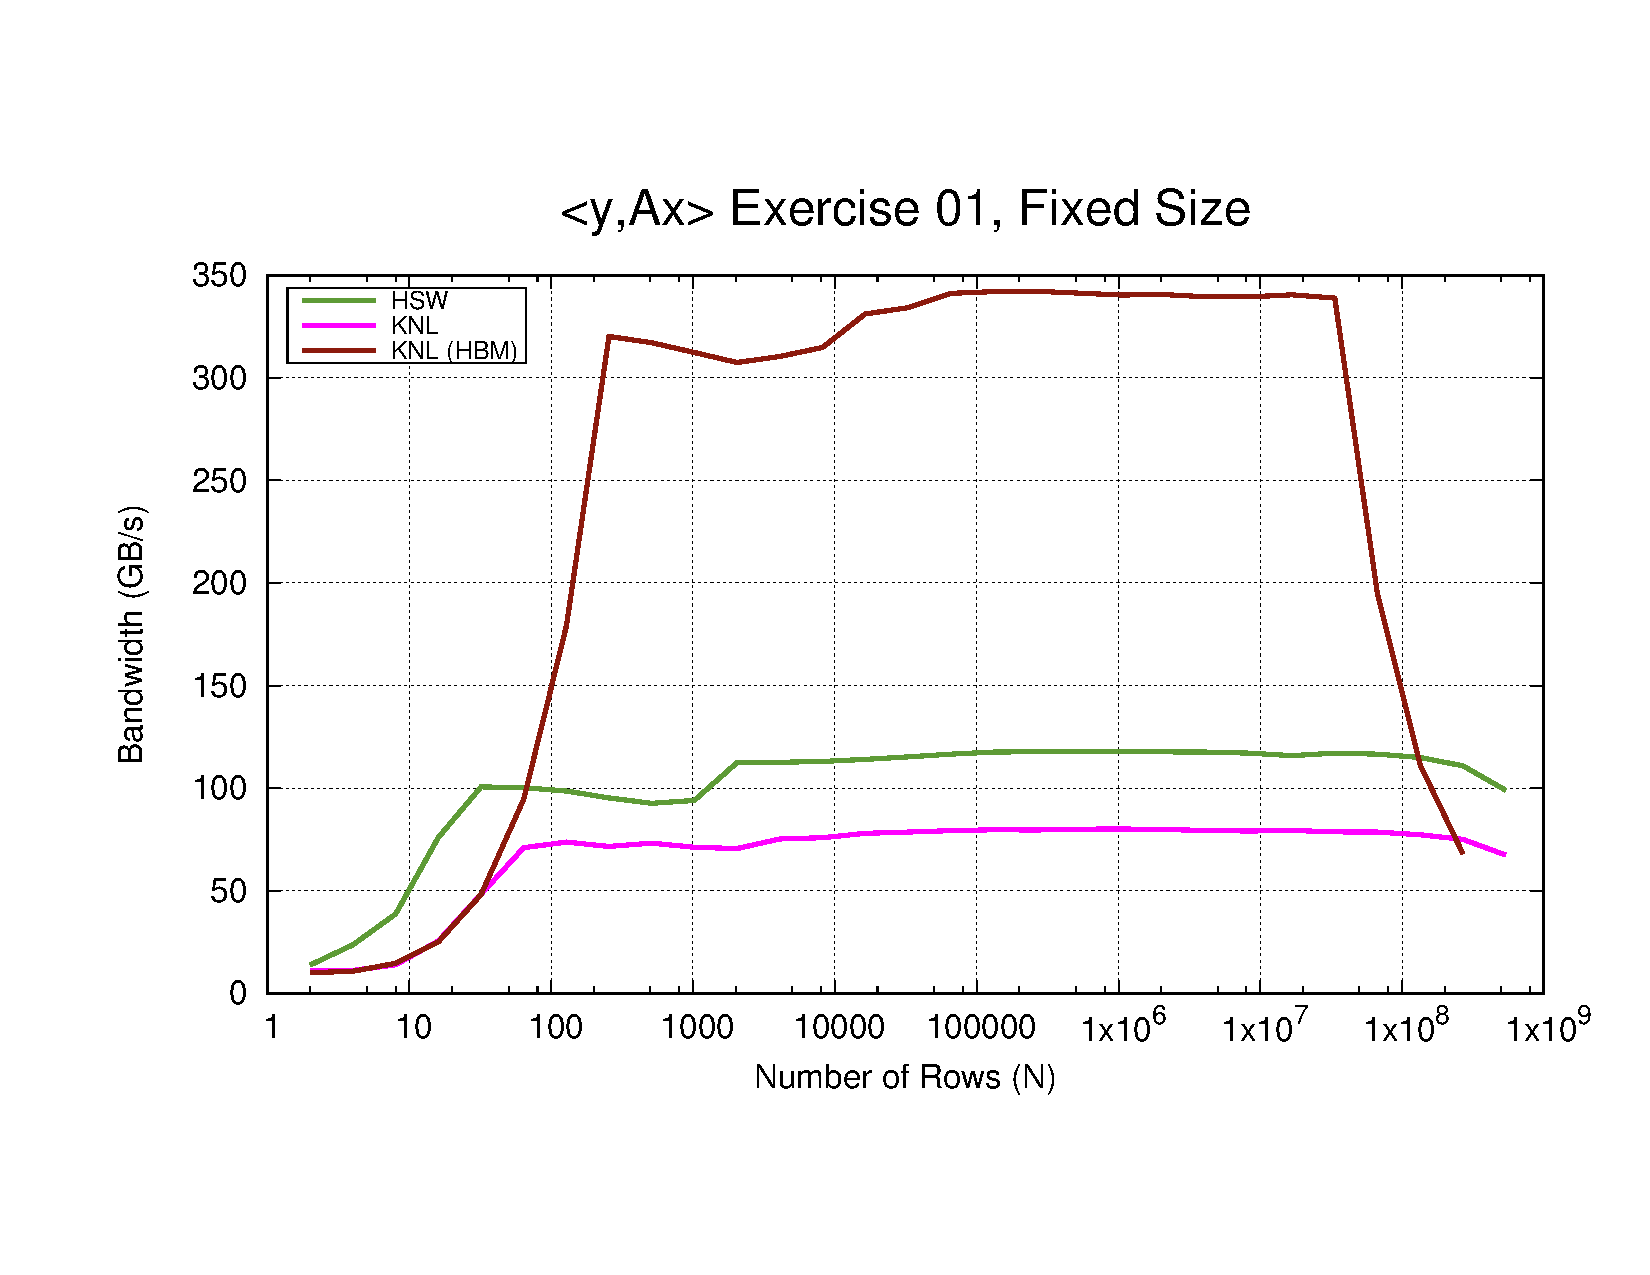
\includegraphics[viewport=1.25in 3.0in 10in 6in, width=1.0\textwidth]{figures/Exercise01-Performance.pdf}
  \end{center}

  \vspace{-15pt}

\end{frame}

%==========================================================================

\iffull
\begin{frame}[fragile]{Exercise \#1 Going beyond}
   \ul{\textbf{More things to try: port your solution to work on the device}}
   \begin{itemize}
     \item You will need to update the dynamic memory allocation.
     \item Replace \texttt{std::malloc} and \texttt{std::free} with \texttt{Kokkos::kokkos\_malloc} and \texttt{Kokkos::kokkos\_free}.
     \item Bonus question:  Why does this perform so poorly?  (hint: the answer is in this slide deck somewhere)
     \item Note that this is just for learning purposes and by no mean a recommended way to manage the lifetime of your arrays.  We will see a better way to do this soon.
   \end{itemize}

   \ul{\textbf{Compiling for GPU}}
  \vspace{-3pt}
  \begin{small}
  \begin{code}
  # if the architecture autodetection fails configure with
  # -DKokkos_ARCH_VOLTA70=ON for V100
  # refer to the documentation for the complete list of supported NVIDIA GPU
  # architectures and corresponding flags, or use ccmake to discover options
    cmake -B build-cuda -DKokkos_ENABLE_CUDA=ON
    cmake --build build-cuda
    make -j KOKKOS_DEVICES=Cuda KOKKOS_ARCH=...
  \end{code}
  \end{small}
\end{frame}
\fi

%==========================================================================

\iffull
\begin{frame}[fragile]{Basic capabilities we haven't covered}

  \begin{itemize}

  \item {Customizing \texttt{parallel\_reduce} data type and reduction operator
    \\ \hspace{10pt} \emph{e.g.}, minimum, maximum, ...}

  \item {\texttt{parallel\_scan} pattern for exclusive and inclusive prefix sum}

  \item {Using \textit{tag dispatch} interface to allow non-trivial functors to have multiple ``\texttt{operator()}'' functions.
    \\ \hspace{10pt} very useful in large, complex applications}

  \end{itemize}

\end{frame}
\fi

%==========================================================================

\begin{frame}{Section Summary}

  \begin{itemize}
    \item{\textbf{Simple} usage is similar to OpenMP, advanced features are also straightforward}
    \item{Three common \textbf{data-parallel patterns} are \texttt{parallel\_for}, \texttt{parallel\_reduce}, and \texttt{parallel\_scan}.}
    \item{A parallel computation is characterized by its \textbf{pattern}, \textbf{policy}, and \textbf{body}.}
    \item{User provides \textbf{computational bodies} as functors or lambdas which handle a single work item.}
  \end{itemize}

\end{frame}


%!TEX root = ../modularized/KokkosTutorial_01_Introduction.tex
% \begin{frame}{DOE ECP Acknowledgement}

% \textit{
% This research was supported by the Exascale Computing Project (17-SC-20-SC),
% a joint project of the U.S. Department of Energy’s Office of Science and National Nuclear Security Administration,
% responsible for delivering a capable exascale ecosystem, including software, applications, and hardware technology,
% to support the nation’s exascale computing imperative. 
% }

% \end{frame}

%==============================================================================

\begin{frame}[fragile]


  \vspace{10pt}
  {\Huge Building Applications with Kokkos}

  \vspace{10pt}

  \textbf{Learning objectives:}
  \begin{itemize}
    \item{Install Kokkos via CMake}
    \item{Build Kokkos inline via CMake}
    \item{Using Spack}
    \item{Build Kokkos inline via GNU Makefiles}
  \end{itemize}

%  \vspace{-20pt}
  \pause

  \begin{block}{Ignore This For Tutorial Only}
     The following details on options to integrate Kokkos into your build process are NOT necessary to know if you just want to do the tutorial.
  \end{block}

\end{frame}

\begin{frame}[fragile]{Options for Building Kokkos}

\begin{itemize}
\item \textbf{Install Kokkos via CMake:} For large projects with multiple dependencies installing Kokkos via CMake and then building against it is the best option.
\item \textbf{Build Kokkos inline via CMake:} This is an option suited for applications which have few dependencies (and no one depending on them) and want to build Kokkos inline with their application.
\item \textbf{Using Spack:} For projects which largely rely on components provided by the Spack package manager.
\item \textbf{Build Kokkos inline via GNU Makefiles:} The option for projects which don't want to use CMake. Only inline builds are supported via Makefiles though. Often this works well for small applications, with few if any dependencies. 
\end{itemize}
\end{frame}

\begin{frame}[fragile]{Kokkos CMake Basics}
\begin{itemize}
\item In the spirit of C++ for \emph{code} performance portability, modern CMake aims for \emph{build system} portability
\item Projects that depend on Kokkos should be agnostic to the exact build configuration of Kokkos
\item No CUDA details in C++! No CUDA details in CMake!
\item Single build system call in your project should configure all compiler/linker flags:

\begin{shell}
add_library(myLib goTeamVenture.cpp)
target_link_libraries(myLib PUBLIC Kokkos::kokkos)
\end{shell}
\item Kokkos configure options are enabled/disabled via CMake as:
\begin{shell}
  cmake -DKokkos_XYZ=ON
\end{shell}
\end{itemize}
\end{frame}

\begin{frame}[fragile]{CMake Backend Options}
\begin{itemize}
\item Numerous backends can be activated 
  \begin{itemize}
    \item Only one GPU, one parallel CPU, and Serial at the same time!
  \end{itemize}
\item \inlineshell{-DKokkos_ENABLE_CUDA=ON}
\item \inlineshell{-DKokkos_ENABLE_HIP=ON}
\item \inlineshell{-DKokkos_ENABLE_SYCL=ON}
\item \inlineshell{-DKokkos_ENABLE_OPENMP=ON}
\begin{uncoverenv}<2->
\item Verify execution spaces in CMake Output, e.g. CUDA
\begin{shell}[linebackground={
  \btLstHL{4}{orange!30}
}]
-- The project name is: Kokkos
...
-- Execution Spaces:
--     Device Parallel: CUDA
--     Host Parallel: NONE
--       Host Serial: SERIAL
\end{shell}
\end{uncoverenv}
\end{itemize}
\end{frame}

\begin{frame}[fragile]{CMake Architecture Options}
\begin{itemize}
\item Device backends \emph{require} architecture be specified (CUDA , OpenMPTarget, and HIP)
\begin{itemize}
  \item \inlineshell{-DKokkos_ARCH_VOLTA70=ON}
  \item \inlineshell{-DKokkos_ARCH_AMD_GFX90A=ON}: MI250X
\end{itemize}
\item Host backends \emph{recommend} architecture be specified to enable architecture-specific optimizations
\begin{itemize}
  \item \inlineshell{-DKokkos_ARCH_HSW=ON}: Haswell
  \item  \inlineshell{-DKokkos_ARCH_ZEN2=ON}: Ryzen (2nd gen)
\end{itemize}
\item Architecture flags will automatically propagate to your project via transitive CMake properties
\begin{uncoverenv}<2->
\item Verify architectures in CMake Output, e.g. Volta 7.0
\begin{shell}[linebackground={
  \btLstHL{4}{orange!30}
}]
-- The project name is: Kokkos
...
-- Architectures:
--  VOLTA70
\end{shell}
\end{uncoverenv}

\end{itemize}
\end{frame}


\begin{frame}[fragile]{CMake And CUDA}
\begin{itemize}
\item Kokkos is a \emph{C++} performance portability layer, but CUDA is usually built as a separate language with \inlineshell{nvcc}.
\item \inlineshell{nvcc} doesn't accept all C++ compiler flags
\item Kokkos' solution for now is to provide  \inlineshell{nvcc_wrapper} that converts \inlineshell{nvcc} into a full C++ compiler.
\uncover<2-> { \item Set CMake C++ compiler to \inlineshell{nvcc_wrapper} }
\uncover<3-> { \item CMake will report compiler as host C++ compiler }
\end{itemize}

\begin{uncoverenv}<2->
\begin{shell}[linebackground={%
    \btLstHL<2>{2}{orange!30}%
}]
> cmake ${KOKKOS_SRC}
  -DCMAKE_CXX_COMPILER=${KOKKOS_SRC}/bin/nvcc_wrapper
  -DKokkos_ENABLE_CUDA=ON
\end{shell}
\end{uncoverenv}

\begin{uncoverenv}<3->
\begin{shell}[linebackground={
   \btLstHL<3>{1}{green!30}%
   \btLstHL<4>{2}{orange!30}
}]
-- The CXX compiler identification is GNU 8.2.0
-- Check for working CXX compiler: bin/nvcc_wrapper
\end{shell}
\end{uncoverenv}

\begin{uncoverenv}<4->
\begin{itemize}
  \item Or simply use clang++ as your compiler...
\end{itemize}
\end{uncoverenv}

\end{frame}

\begin{frame}[fragile]{CMake And HIP}

\textbf{Enable HIP backend}
Configure with:
\begin{lstlisting}[language=bash]
-DKokkos_ENABLE_HIP=ON
\end{lstlisting}

\textbf{Compiler}
 Need to explicitly set \texttt{hipcc} or \texttt{amdclang++} as C++ compiler:
\begin{lstlisting}[language=bash]
-DCMAKE_CXX_COMPILER=hipcc
\end{lstlisting}

\textbf{Architecture flags}
Chose one from:
\begin{lstlisting}[language=bash]
-DKokkos_ARCH_AMD_GFX908=ON # for AMD Radeon Instinct MI100
-DKokkos_ARCH_AMD_GFX90A=ON # for AMD Radeon Instinct MI200 series
\end{lstlisting}

\end{frame}

\begin{frame}[fragile]{CMake And SYCL}

\textbf{Enable SYCL backend}
Configure with:
\begin{lstlisting}[language=bash]
-DKokkos_ENABLE_SYCL=ON
\end{lstlisting}

\textbf{Compiler}
 Need to explicitly set \texttt{icpx} as C++ compiler:
\begin{lstlisting}[language=bash]
-DCMAKE_CXX_COMPILER=icpx
\end{lstlisting}

\textbf{Architecture flags}
Chose one from:
\begin{lstlisting}[language=bash]
-DKokkos_ARCH_INTEL_GEN=ON # JIT compiler
-DKokkos_ARCH_INTEL_PVC=ON # for GPU Max 1550/Ponte Vecchio
\end{lstlisting}

\end{frame}

\begin{frame}[fragile]{CMake And OpenMPTarget}
\begin{itemize}
\item Similar configuration as CUDA/HIP backends, but use:
\begin{shell}
cmake -DKokkos_ENABLE_OPENMPTARGET=ON
\end{shell}
\item Still requires target device architecture to be given:
\begin{shell}
cmake -DKokkos_ARCH_VOLTA70=ON
\end{shell}
\item Currently very sensitive to exact compiler/STL combination
\begin{itemize}
\item Clang15+
\item GCC9 Toolchain
\item See \url{scripts/docker/Dockerfile.openmptarget} for recipe
\end{itemize}
\item C++17 is required
\item Working on Spack packages to handle complex version dependencies
\end{itemize}
\end{frame}

\begin{frame}[fragile]{Building Against an Installed Kokkos (i)}

Find exported Kokkos configuration (include dirs, libraries to link against, compile options, etc.)
and generate my project's build system accordingly.

\textbf{Basic starting point}
Create a \texttt{CMakeLists.txt} file.
\begin{lstlisting}[language=bash]
cmake_minimum_required(VERSION 3.16)
project(myProject CXX) # C++ needed to build my project

find_package(Kokkos REQUIRED) # fail if Kokkos not found

# build my executable from the specified source code
add_executable(myExe source.cpp)
# declare dependency on Kokkos
target_link_libraries(myExe PRIVATE Kokkos::kokkos)
\end{lstlisting}

\textbf{Working with a library}
\begin{lstlisting}[language=bash]
find_package(Kokkos 4.0 REQUIRED) # request Kokkos minimum version
add_library(myLib ${SOURCES})
target_link_libraries(myLib PUBLIC Kokkos::kokkos)
\end{lstlisting}

\end{frame}

\begin{frame}[fragile]{Building Against an Installed Kokkos (ii)}

\textbf{Finding Kokkos} Add Kokkos installation prefix to the list of directories searched by CMake:
\begin{lstlisting}[language=bash]
cmake .. -DKokkos_ROOT=<prefix> -DCMAKE_CXX_COMPILER=<...>
\end{lstlisting}

\textbf{Kokkos package introspection}
Assert that support for \texttt{\_\_host\_\_}, \texttt{\_\_device\_\_} annotations in lambdas declaration is enabled
\begin{lstlisting}[language=bash]
# (optional) assume my project uses lambdas
if(Kokkos_ENABLE_CUDA)
  # fatal error if not enabled
  kokkos_check(OPTIONS CUDA_ENABLE_LAMBDA)
endif()
\end{lstlisting}
or query that generation of relocatable device code is enabled
\begin{lstlisting}[language=bash]
kokkos_check(
  DEVICES CUDA
  OPTIONS CUDA_RELOCATABLE_DEVICE_CODE
  RESULT_VARIABLE KOKKOS_HAS_CUDA_RDC)
if(KOKKOS_HAS_CUDA_RDC)
  ...
\end{lstlisting}

\end{frame}


\begin{frame}[fragile]{CMake Building Kokkos Inline}
Build Kokkos as part of your own project (as opposed to finding a pre-installed Kokkos)
\begin{lstlisting}[language=bash]
add_subdirectory(<kokkos source dir>)

# identical as when finding an installed Kokkos package
add_executable(myExe ${SOURCES})
target_link_libraries(myExe PRIVATE Kokkos::kokkos)
\end{lstlisting}

Pass Kokkos options along with app-specific options at configuration time
\begin{lstlisting}[language=bash]
cmake .. -DCMAKE_CXX_COMPILER=<kokkos dir>/bin/nvcc_wrapper \
  -DKokkos_ENABLE_CUDA=ON -DKokkos_ENABLE_CUDA_LAMBDA=ON \
  -DmyApp_ENABLE_FOO=ON -DmyApp_ENABLE_BAR=ON
\end{lstlisting}

\end{frame}

\begin{frame}[fragile]{Kokkos via Spack: Command Line}
\begin{itemize}
\item Spack provides a package manager that automatically downloads, configures, and installs package dependencies
\item Kokkos itself can be easily installed with specific variants (+) and compilers (\%)
\begin{shell}
spack install kokkos@develop +openmp %gcc@8.3.0
\end{shell}
\item Good practice is to define ``best variant`` in your packages.yaml directory, e.g. for Volta system
\begin{shell}
packages:
   kokkos:
    variants: +cuda +openmp +cuda_lambda +wrapper \
              ^cuda@12.0 cuda_arch=70
    compiler: [gcc@8.3.0]
\end{shell}
\item Build rules in \inlineshell{package.py} automatically map Spack variants to correct CMake options
\item Run \inlineshell{spack info kokkos} to see full list of variants
\end{itemize}
\end{frame}

\begin{frame}[fragile]{Kokkos via Spack: Package Files}
\begin{itemize}
\item Build rules created in a \inlineshell{package.py} file
\item Step 1: Declare dependency on specific version of kokkos (3.x, master, or develop)
\begin{shell}
class myLib(CMakePackage):
  depends_on('kokkos@3.2')
\end{shell}
\item Step 2: Add build rule pointing to Spack-installed Kokkos and same C++ compiler Kokkos uses
\begin{shell}
def cmake_args(self):
  options = []
  ...
  options.append('-DCMAKE_CXX_COMPILER={}'.format(
     self.spec['kokkos'].kokkos_cxx)
  options.append('-DKokkos_ROOT={}'.format(
     self.spec['kokkos'].prefix)
  return options
\end{shell}
\item Full details can be found in Spack.md in Kokkos repo.
\end{itemize}
\end{frame}

\begin{frame}[fragile]{Building Kokkos Inline via GNU Makefiles}
	\textbf{Building Kokkos inline with GNU Makefiles in three steps:}

        \begin{itemize}
	        \item Set Kokkos Options e.g. \texttt{KOKKOS\_DEVICES}, \texttt{KOKKOS\_ARCH}
		\item Include \texttt{Makefile.kokkos}
		\item Add \texttt{KOKKOS\_CXXFLAGS, KOKKOS\_LDFLAGS} etc. to build rules
	\end{itemize}

	\textbf{Most Important Settings:}

	\begin{itemize}
	   \item \texttt{KOKKOS\_DEVICES}: What backends to enabled. Comma separated list: \texttt{Serial,OpenMP,Cuda,HIP,OpenMPTarget}
	   \item \texttt{KOKKOS\_ARCH}: Set architectures. Comma separated list: \texttt{HSW,Volta70,Power9,...}
	\end{itemize}

	\pause
	\begin{block}{Order Matters!}
	   Add default target, Kokkos settings, and CXXFLAGS before including Makefile.kokkos!
	\end{block}
\end{frame}

\begin{frame}[fragile]{Example Makefile}
\begin{tiny}
\begin{shell}
KOKKOS_PATH = ${HOME}/Kokkos/kokkos
SRC = $(wildcard *.cpp)
KOKKOS_DEVICES=OpenMP,Cuda
KOKKOS_ARCH = SKX,Volta70

default: test
  echo "Start Build"

CXX = clang++
CXXFLAGS = -O3 -g
LINK = ${CXX}

OBJ = $(SRC:.cpp=.o)

include $(KOKKOS_PATH)/Makefile.kokkos

test: $(OBJ) $(KOKKOS_LINK_DEPENDS)
  $(LINK) $(KOKKOS_LDFLAGS) $(OBJ) $(KOKKOS_LIBS) -o test

%.o:%.cpp $(KOKKOS_CPP_DEPENDS)
  $(CXX) $(KOKKOS_CPPFLAGS) $(KOKKOS_CXXFLAGS) $(CXXFLAGS)  -c $<
\end{shell}
\end{tiny}
\end{frame}


\begin{frame}{Section Summary}

  \begin{itemize}
    \item{Kokkos' primary build system is CMAKE.}
    \item{Kokkos options are transitively passed on, including many necessary compiler options.}
    \item{The Spack package manager does support Kokkos.}
    \item{If you write an application, and have few if any dependencies, building Kokkos as part of your code is an option with both CMake and GNU Makefiles.}
  \end{itemize}

\end{frame}


\begin{frame}{Module 1: Summary}
	\textbf{Kokkos Ecosystem:}
	\begin{itemize}
		\item C++ Performance Portability Programming Model.
		\item The Kokkos Ecosystem provides capabilities needed for serious code development.
		\item Kokkos is supported by multiple National Laboratories with a sizeable dedicated team.
	\end{itemize}

	\textbf{Building Kokkos}
	\begin{itemize}
    \item{Kokkos' primary build system is CMAKE.}
    \item{Kokkos options are transitively passed on, including many necessary compiler options.}
    \item{The Spack package manager does support Kokkos.}
    \item{For applications with few if any dependencies, building Kokkos as part of your code is an option with CMake and GNU Makefiles.}
	\end{itemize}
\end{frame}

\begin{frame}[fragile]{Module 1: Summary}
	\textbf{Data Parallelism:}
	\begin{itemize}
		\item Simple things stay simple!
		\item You use \textbf{parallel patterns} and \textbf{execution policies} to execute \textbf{computational bodies}
		\item Simple parallel loops use the \texttt{parallel\_for} pattern:
\begin{code}[linebackgroundcolor={\btLstHL<1->{3}{bodyColor}},frame=single]
  @patternparallel_for@pattern("Label",@policyN@policy, [=] (int64_t i) {
   /* loop body */
  });
\end{code}
\item Reductions combine contributions from loop iterations
\begin{code}[linebackgroundcolor={\btLstHL<1->{3}{bodyColor}},frame=single]
int result;
@patternparallel_reduce@pattern("Label",@policyN@policy, [=] (int64_t i, int& lres) {
   /* loop body */
    lres += /* something */
  },result);
\end{code}
\end{itemize}

\end{frame}


\begin{frame}{Module 2: Outlook (07/24)}

	\vspace{10pt}
	\textbf{Kokkos::View:}
	\begin{itemize}
		\item Solving the data-layout issue.
		\item Controlling data life-time.
	\end{itemize}

	\vspace{10pt}
	\textbf{Execution and Memory Spaces:}
	\begin{itemize}
		\item How to control where data lives.
		\item How to control where code executes.
		\item How to manage data transfers.
	\end{itemize}

	\vspace{10pt}
    \textbf{Slack channel:} {\scriptsize \url{https://kokkosteam.slack.com/}}
	
	\vspace{10pt}
	\textbf{Recordings/Slides:} {\scriptsize \url{https://kokkos.org/kokkos-core-wiki/videolectures.html}}

\end{frame}

\end{document}

